%
\hsection{Installing PostgreSQL under Ubuntu Linux}%
%
\begin{figure}%
\centering%
%
\subfloat[][%
Installing \postgresql\ using the \bashil{apt-get install} command in a \pgls{terminal} opened with \ubuntuTerminal.%
\label{fig:installingPostgresUbuntu01aptGet}%
]{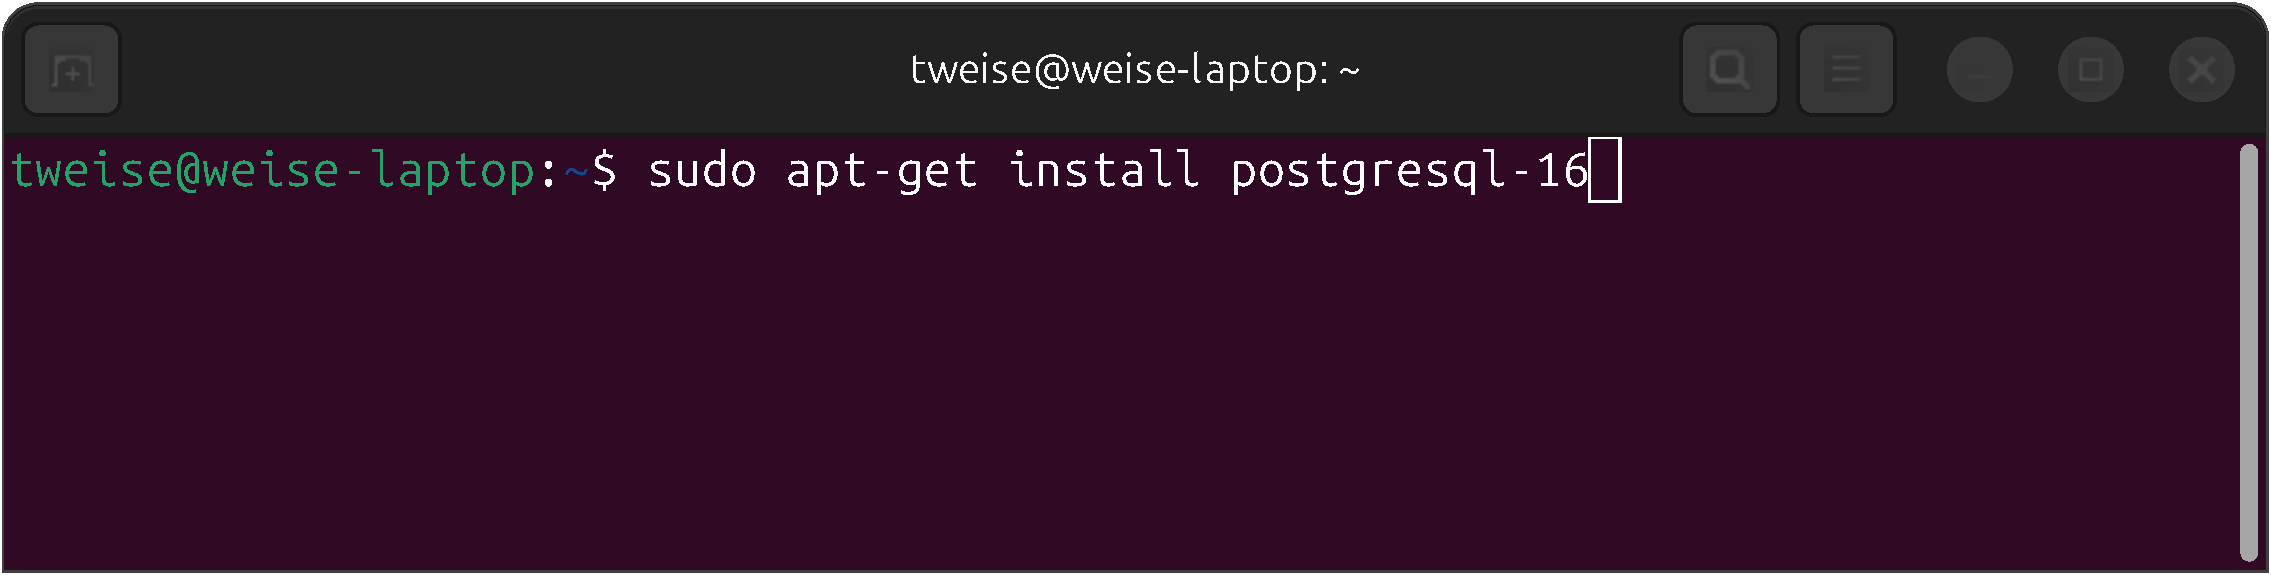
\includegraphics[width=0.7\linewidth]{\currentDir/installingPostgresUbuntu01aptGet}}%
%
\floatRowSep
%
\subfloat[][%
This command requires the super user password, which we type in and then press~\keys{\enter}.%
\label{fig:installingPostgresUbuntu02pass}%
]{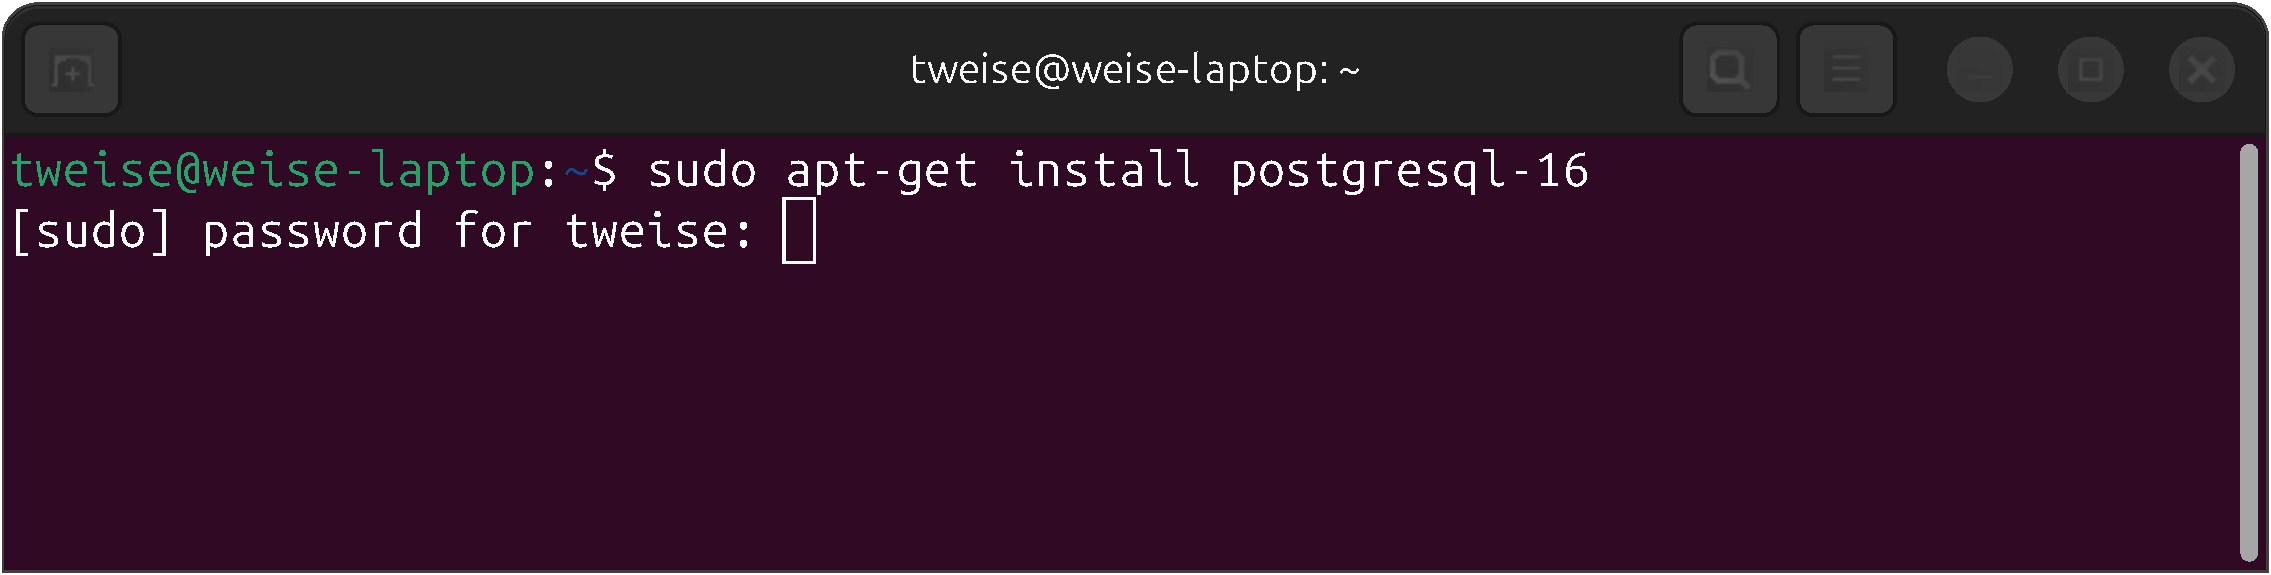
\includegraphics[width=0.7\linewidth]{\currentDir/installingPostgresUbuntu02pass}}%
%
\floatRowSep
%
\subfloat[][%
We get asked whether we really want to install the required packages.%
\label{fig:installingPostgresUbuntu03yn}%
]{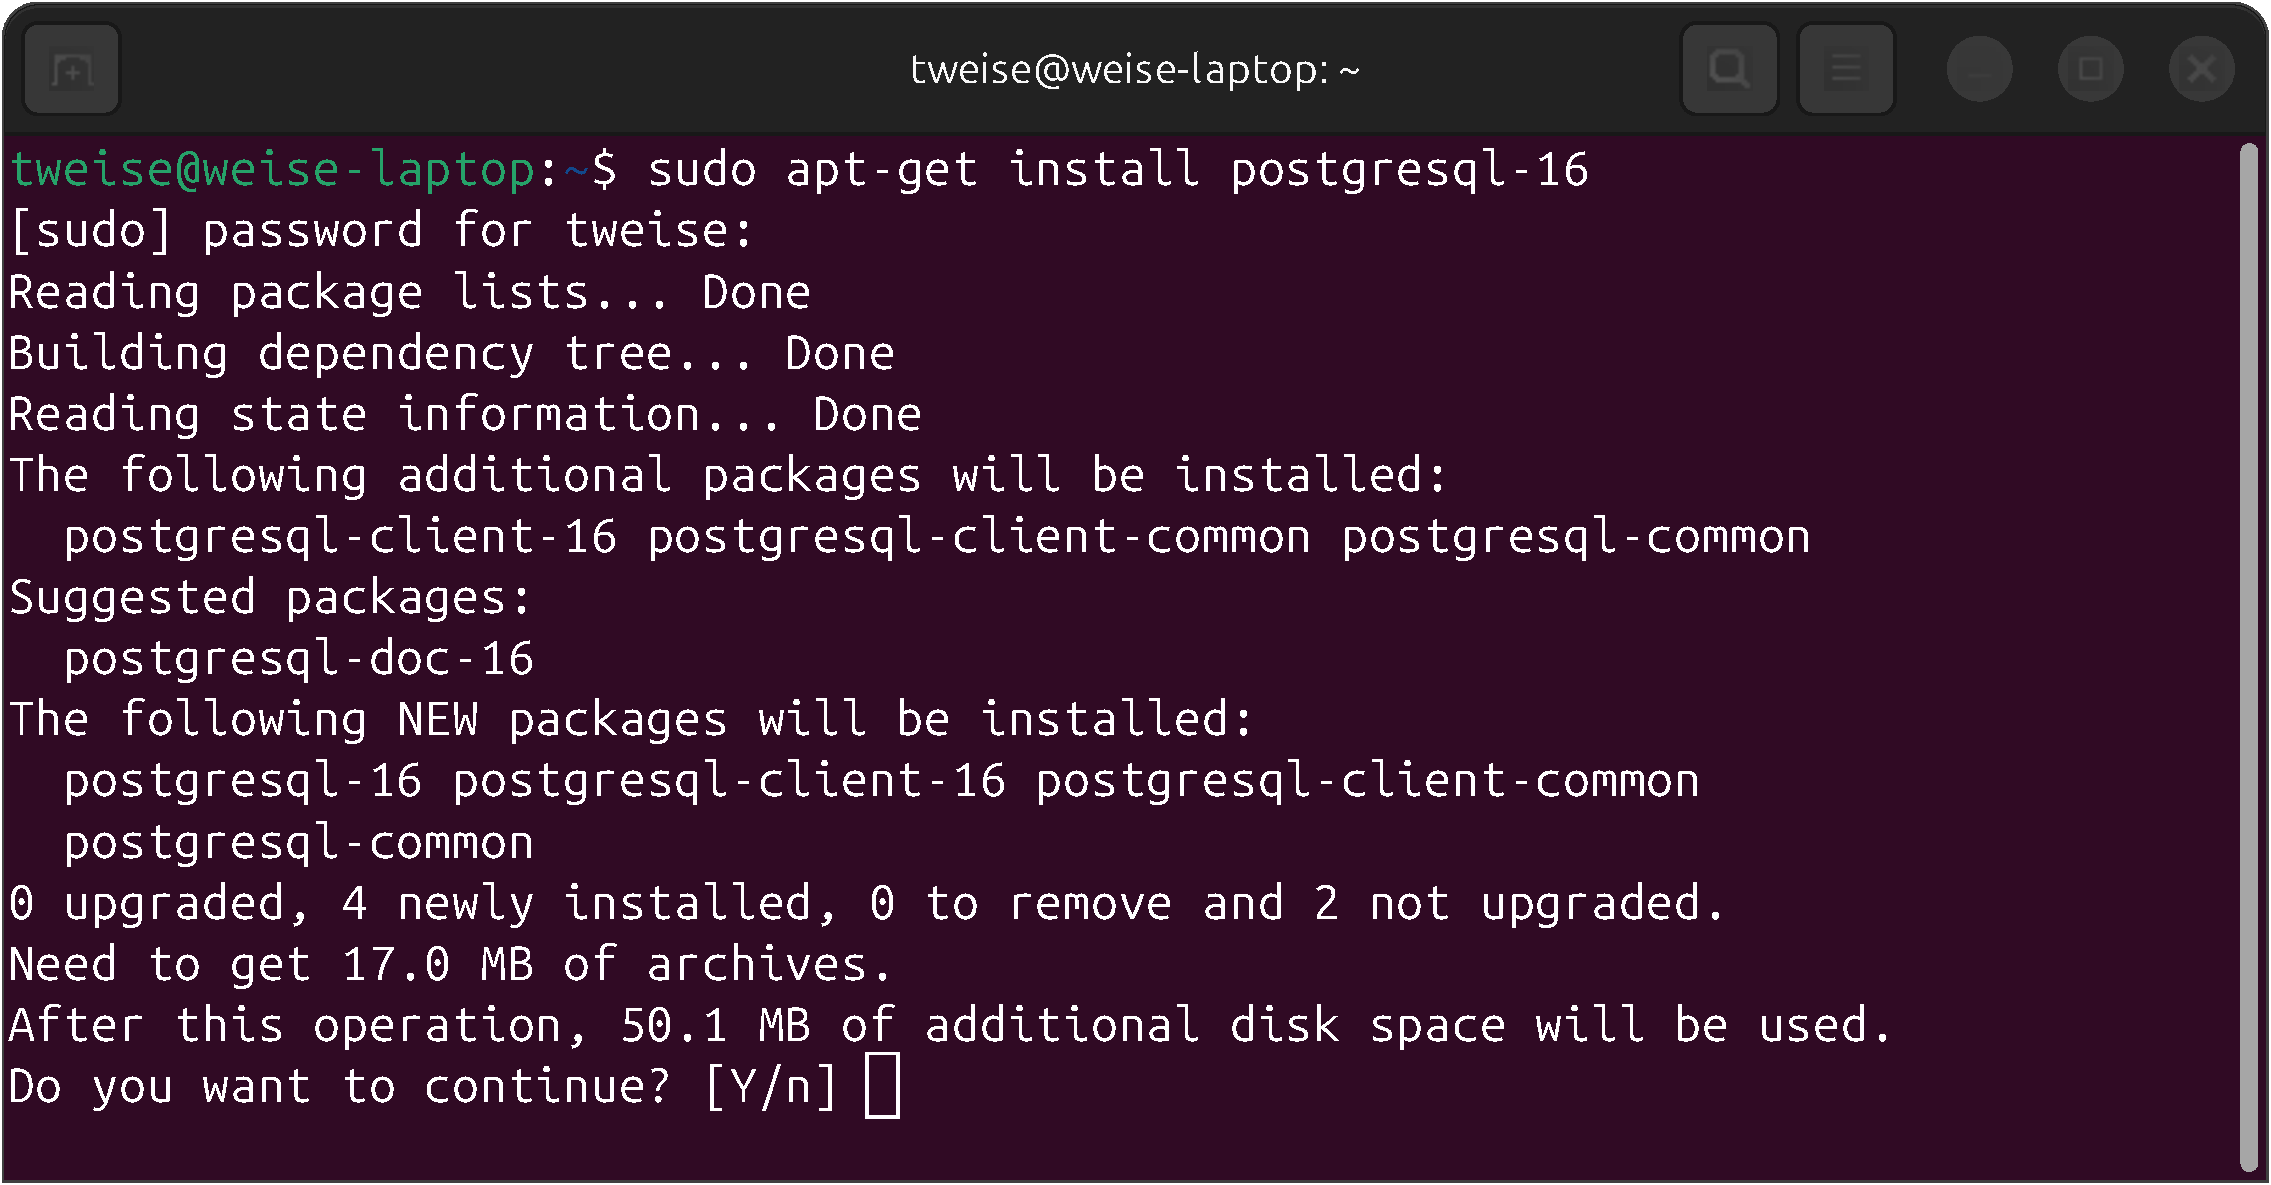
\includegraphics[width=0.7\linewidth]{\currentDir/installingPostgresUbuntu03yn}}%
%
\floatRowSep
%
\subfloat[][%
We answer with~\keys{y+\enter}.%
\label{fig:installingPostgresUbuntu04yny}%
]{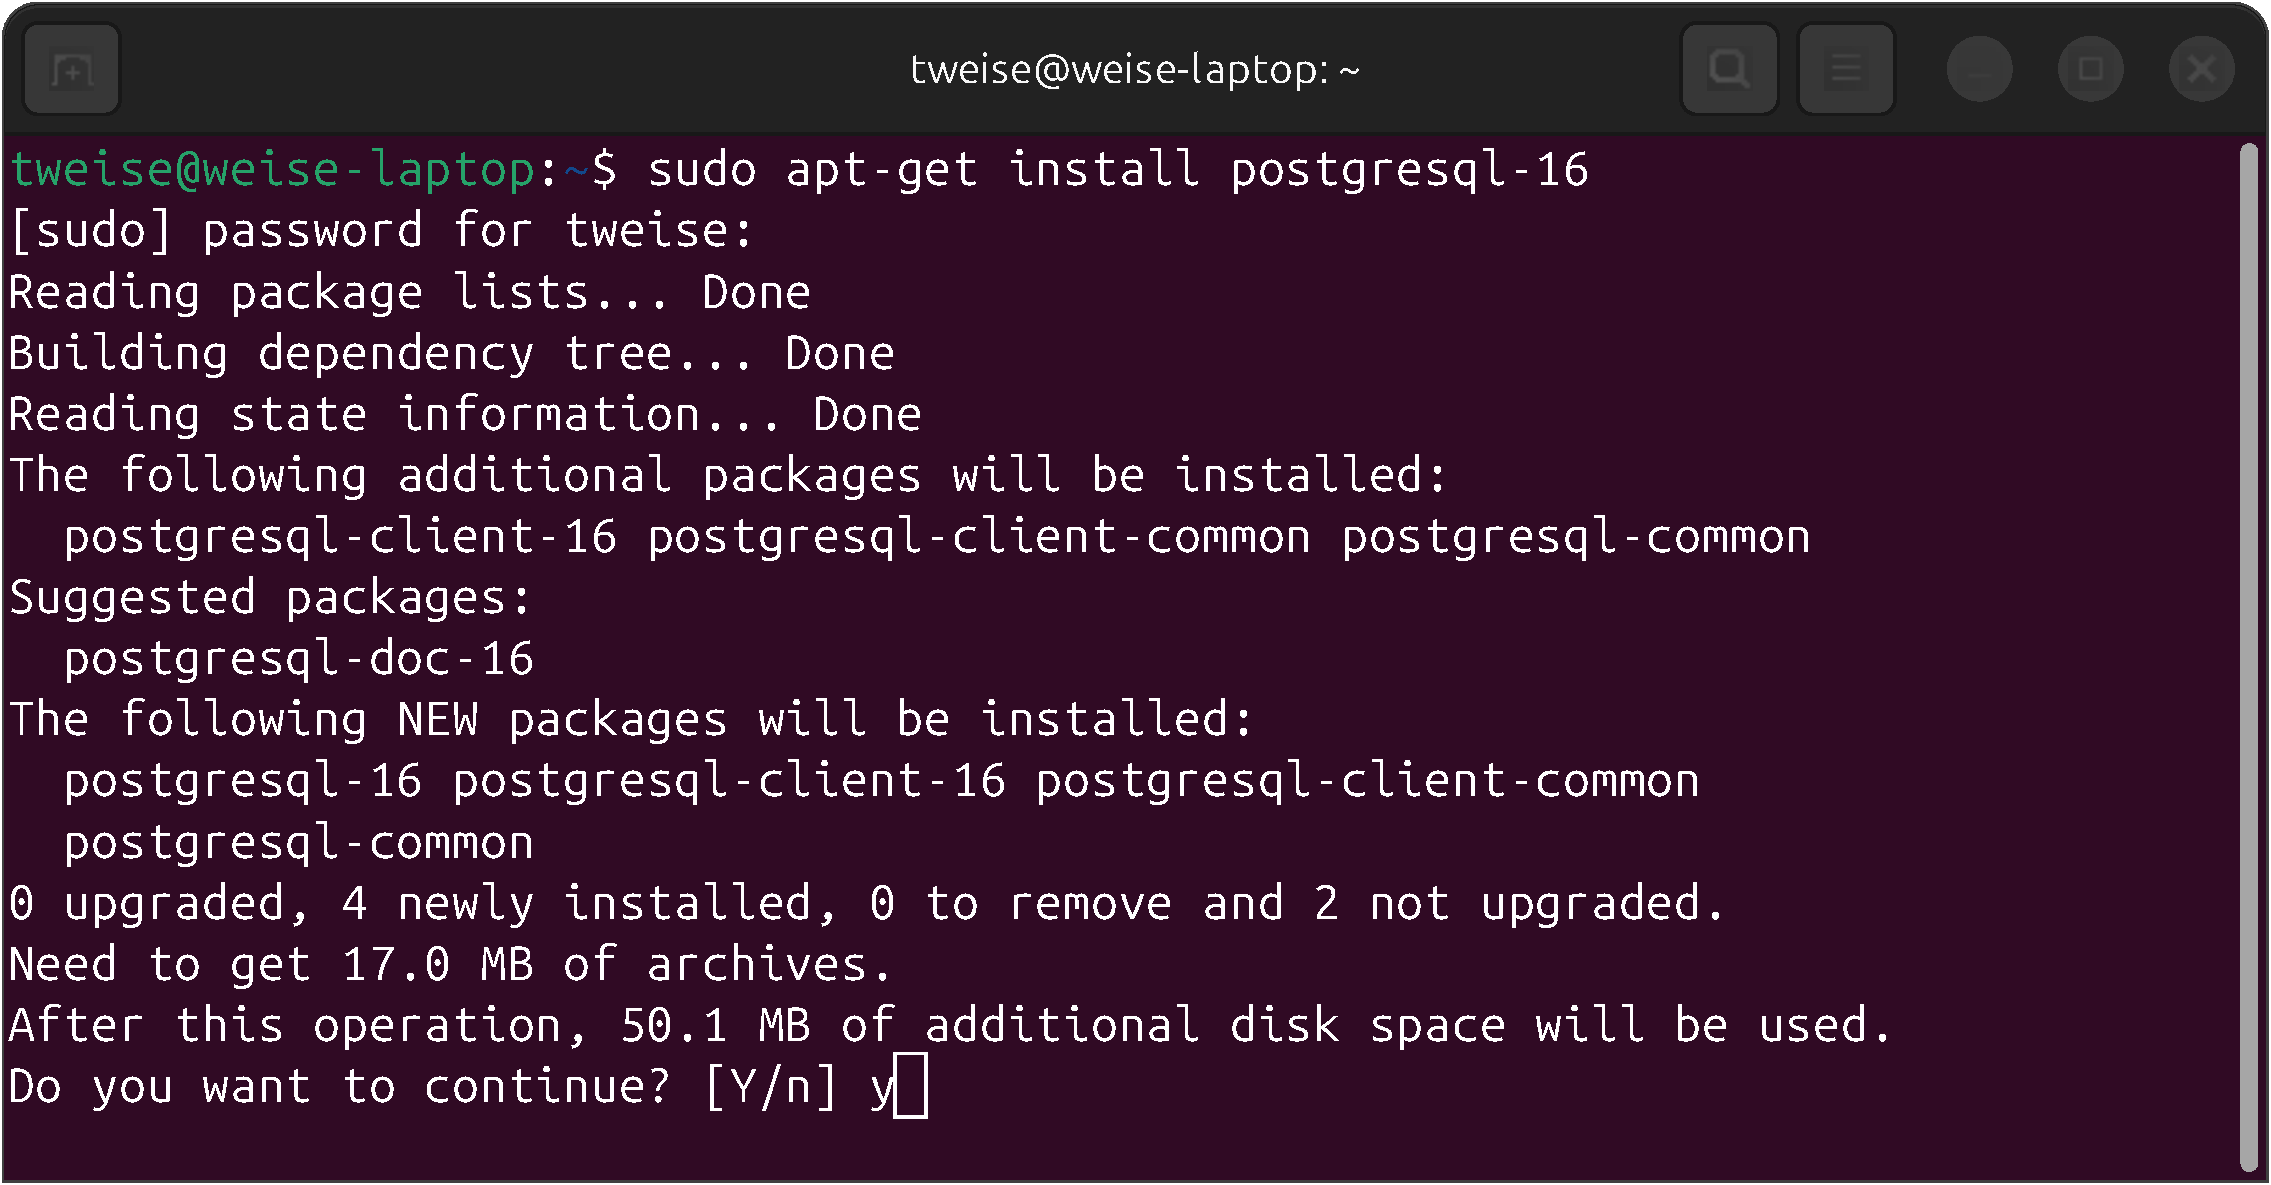
\includegraphics[width=0.7\linewidth]{\currentDir/installingPostgresUbuntu04yny}}%
%
%
\caption{Installing \postgresql\ under \ubuntu\ \linux, checking its status, and setting a secure password.}%
\label{fig:installingPostgresUbuntuA}%
%
\end{figure}%
%
%
\begin{figure}%
\ContinuedFloat
\centering%
%
\subfloat[][%
The installation proceeds and finishes.%
\label{fig:installingPostgresUbuntu05install}%
]{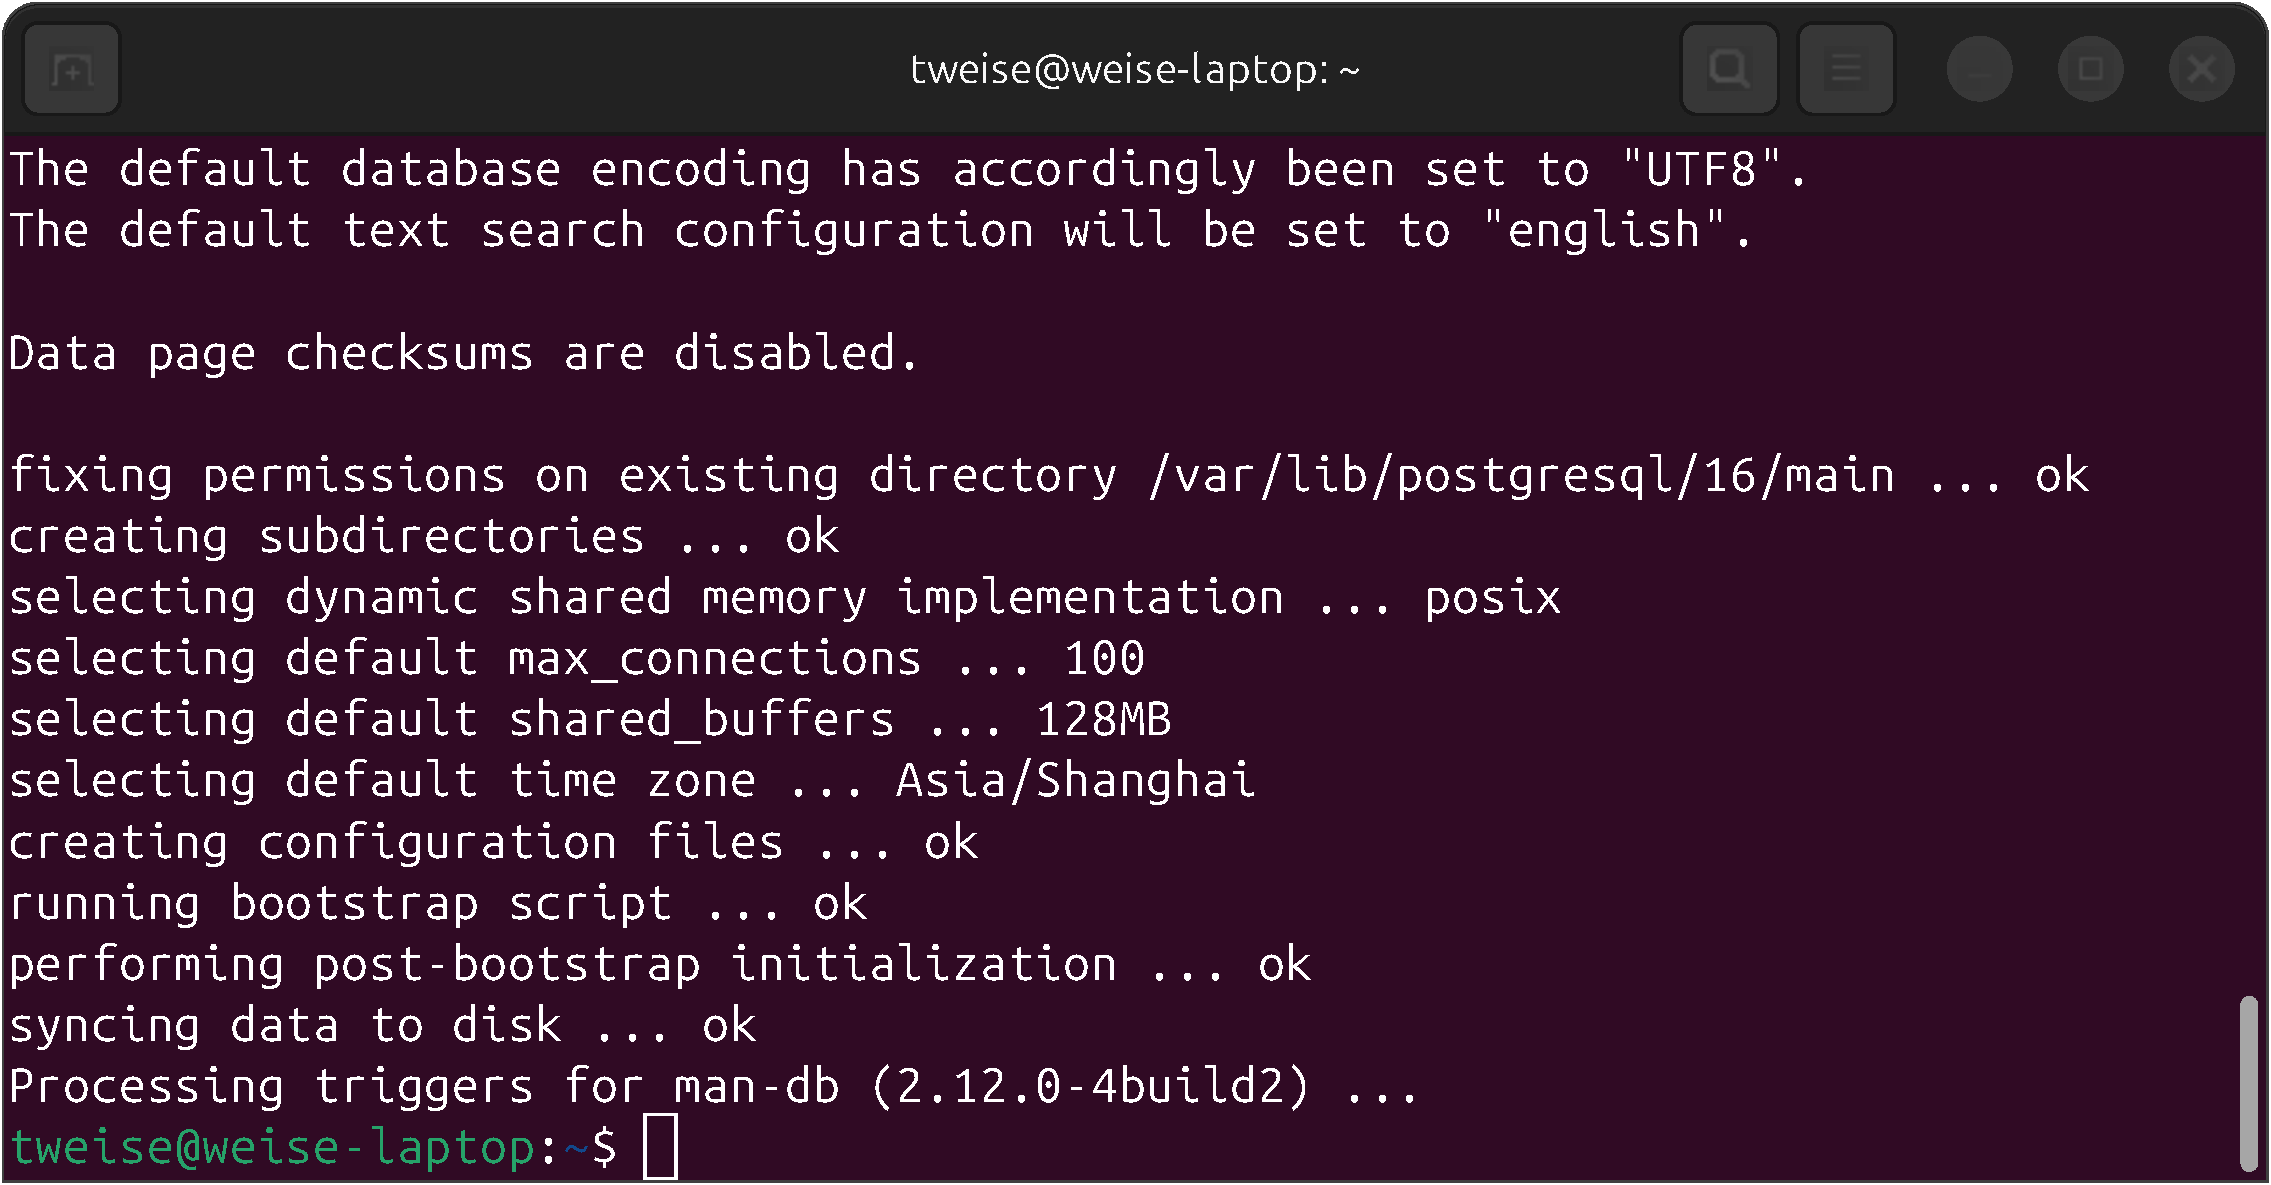
\includegraphics[width=0.7\linewidth]{\currentDir/installingPostgresUbuntu05install}}%
%
\floatRowSep
%
\subfloat[][%
We want to check the status of the fresh \postgresql\ installation. %
We can do this by typing in \bashil{systemctl status postgresql} and hit~\keys{\enter}.%
\label{fig:installingPostgresUbuntu06systemctlCheckStatus}%
]{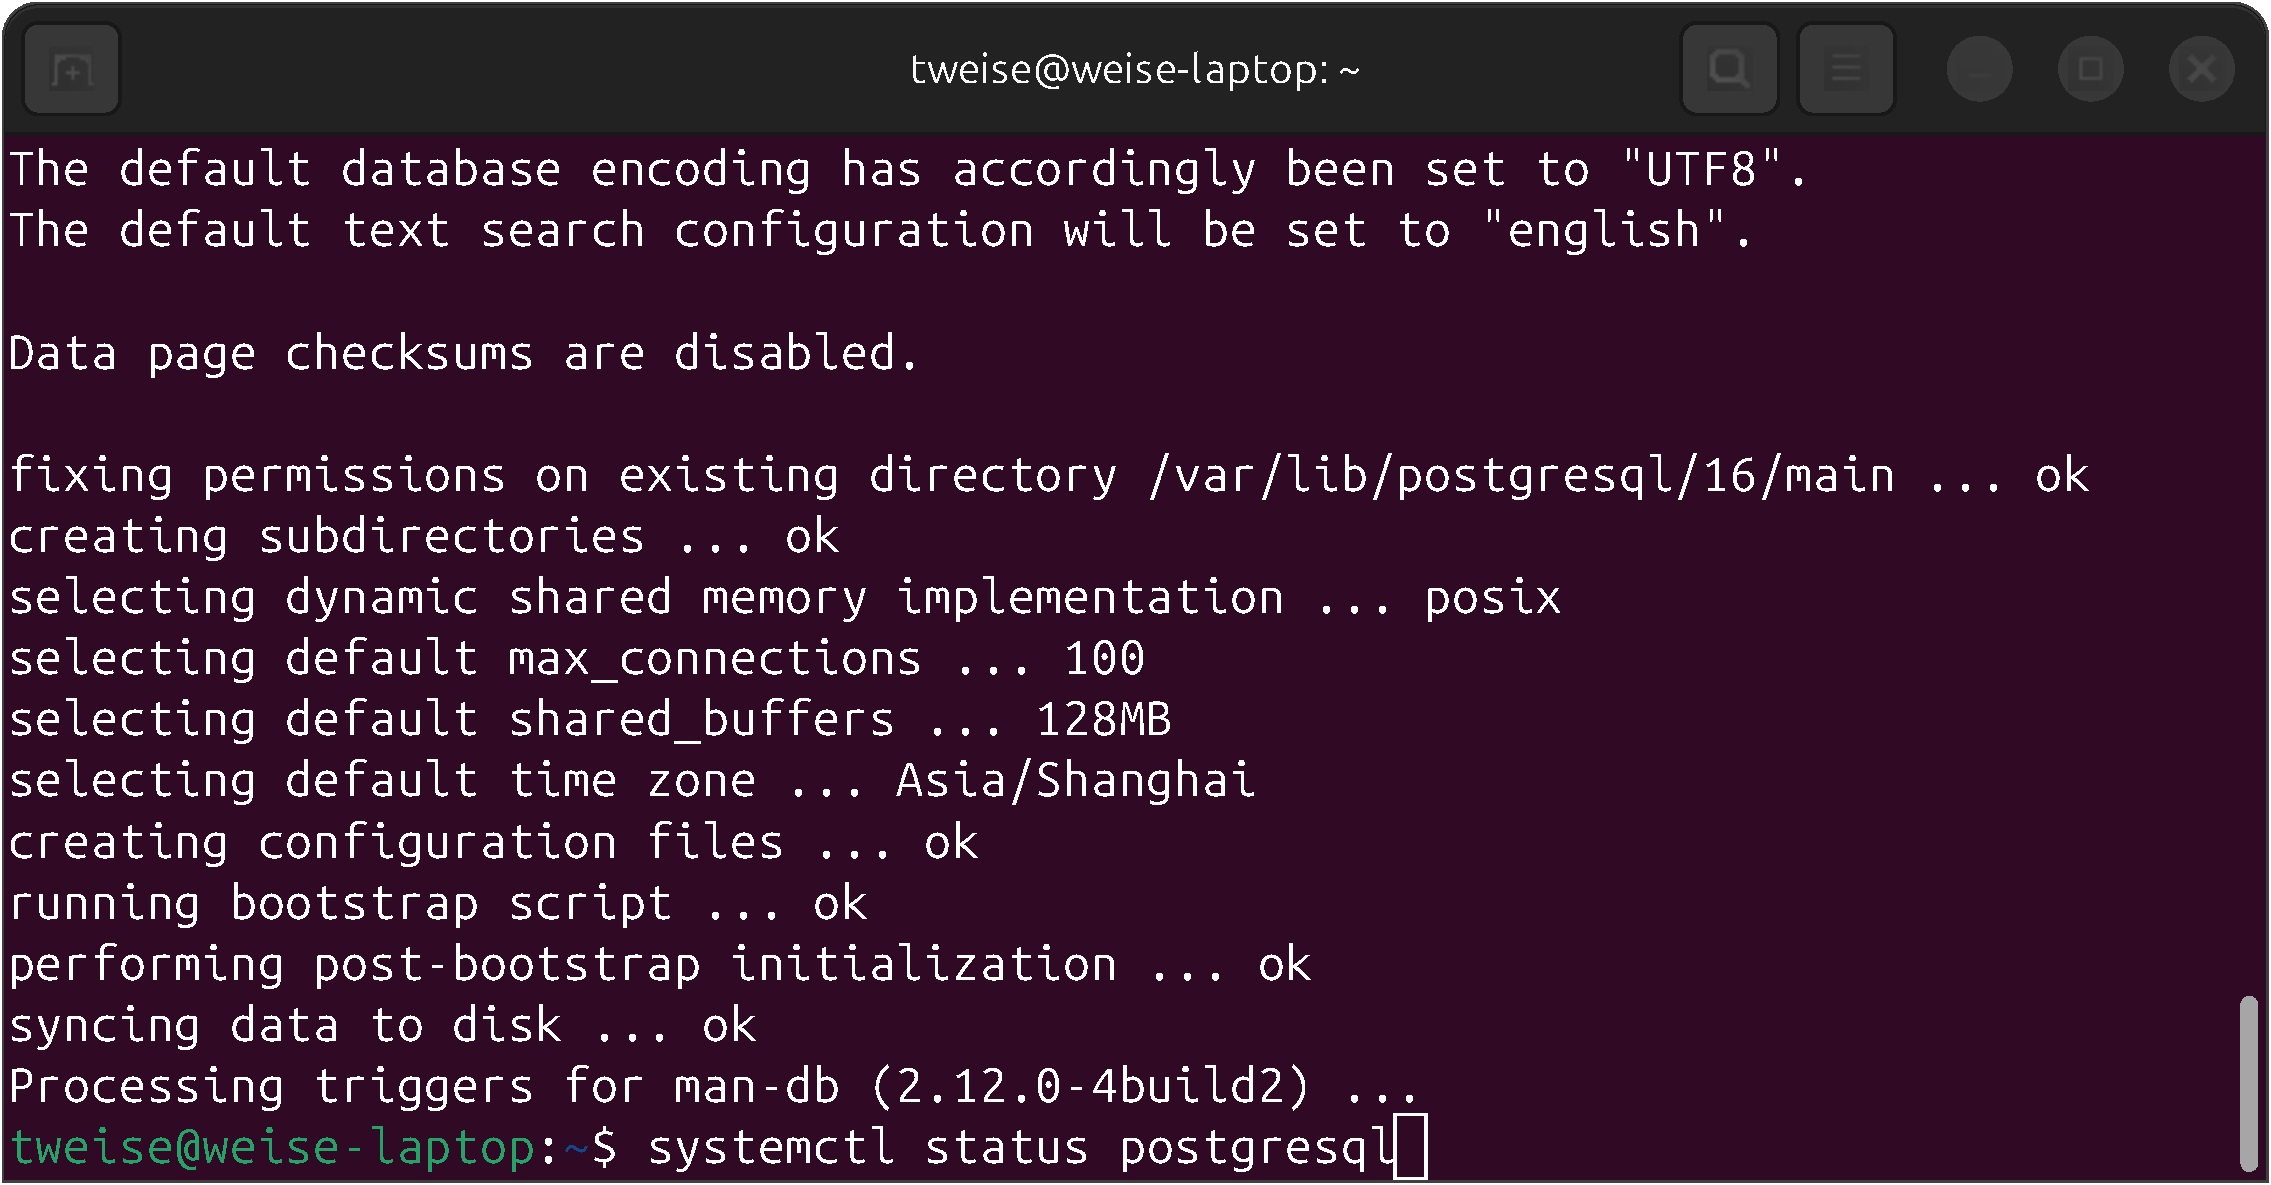
\includegraphics[width=0.7\linewidth]{\currentDir/installingPostgresUbuntu06systemctlCheckStatus}}%
%
\floatRowSep
%
\subfloat[][%
The output shows us that the \postgresql\ service is now running. %
It will always start when we boot our system.%
\label{fig:installingPostgresUbuntu07systemctlCheckStatusRes}%
]{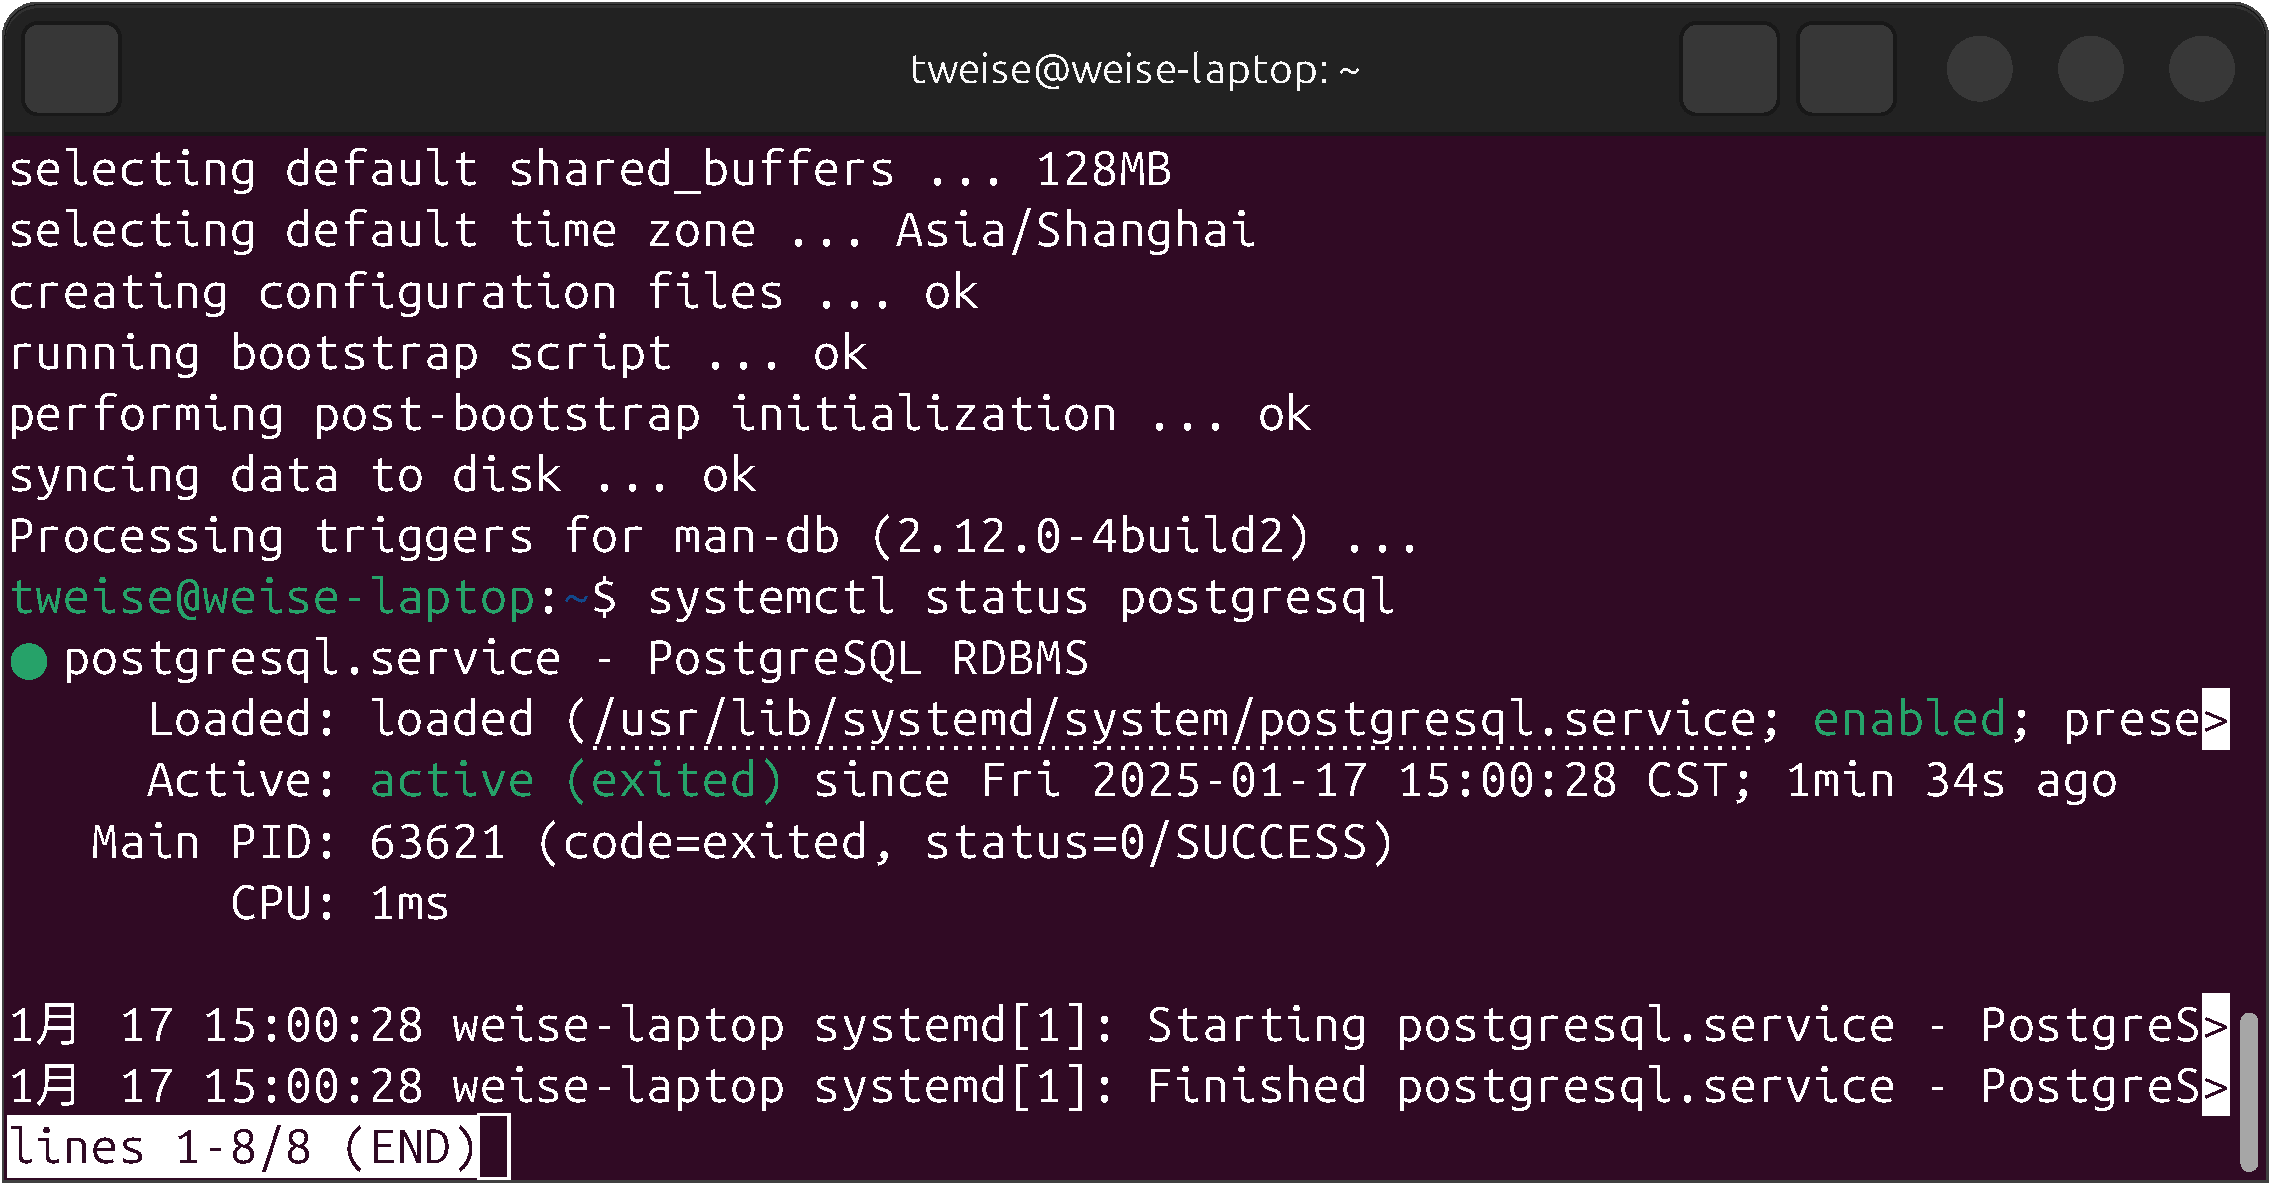
\includegraphics[width=0.7\linewidth]{\currentDir/installingPostgresUbuntu07systemctlCheckStatusRes}}%
%
%
\caption{Installing \postgresql\ under \ubuntu\ \linux, checking its status, and setting a secure password.}%
\label{fig:installingPostgresUbuntuB}%
%
\end{figure}%
%
%
\begin{figure}%
\ContinuedFloat
\centering%
%
\subfloat[][%
We press~\keys{q+\enter} to leave the status output page.%
\label{fig:installingPostgresUbuntu08systemctlCheckStatusQ}%
]{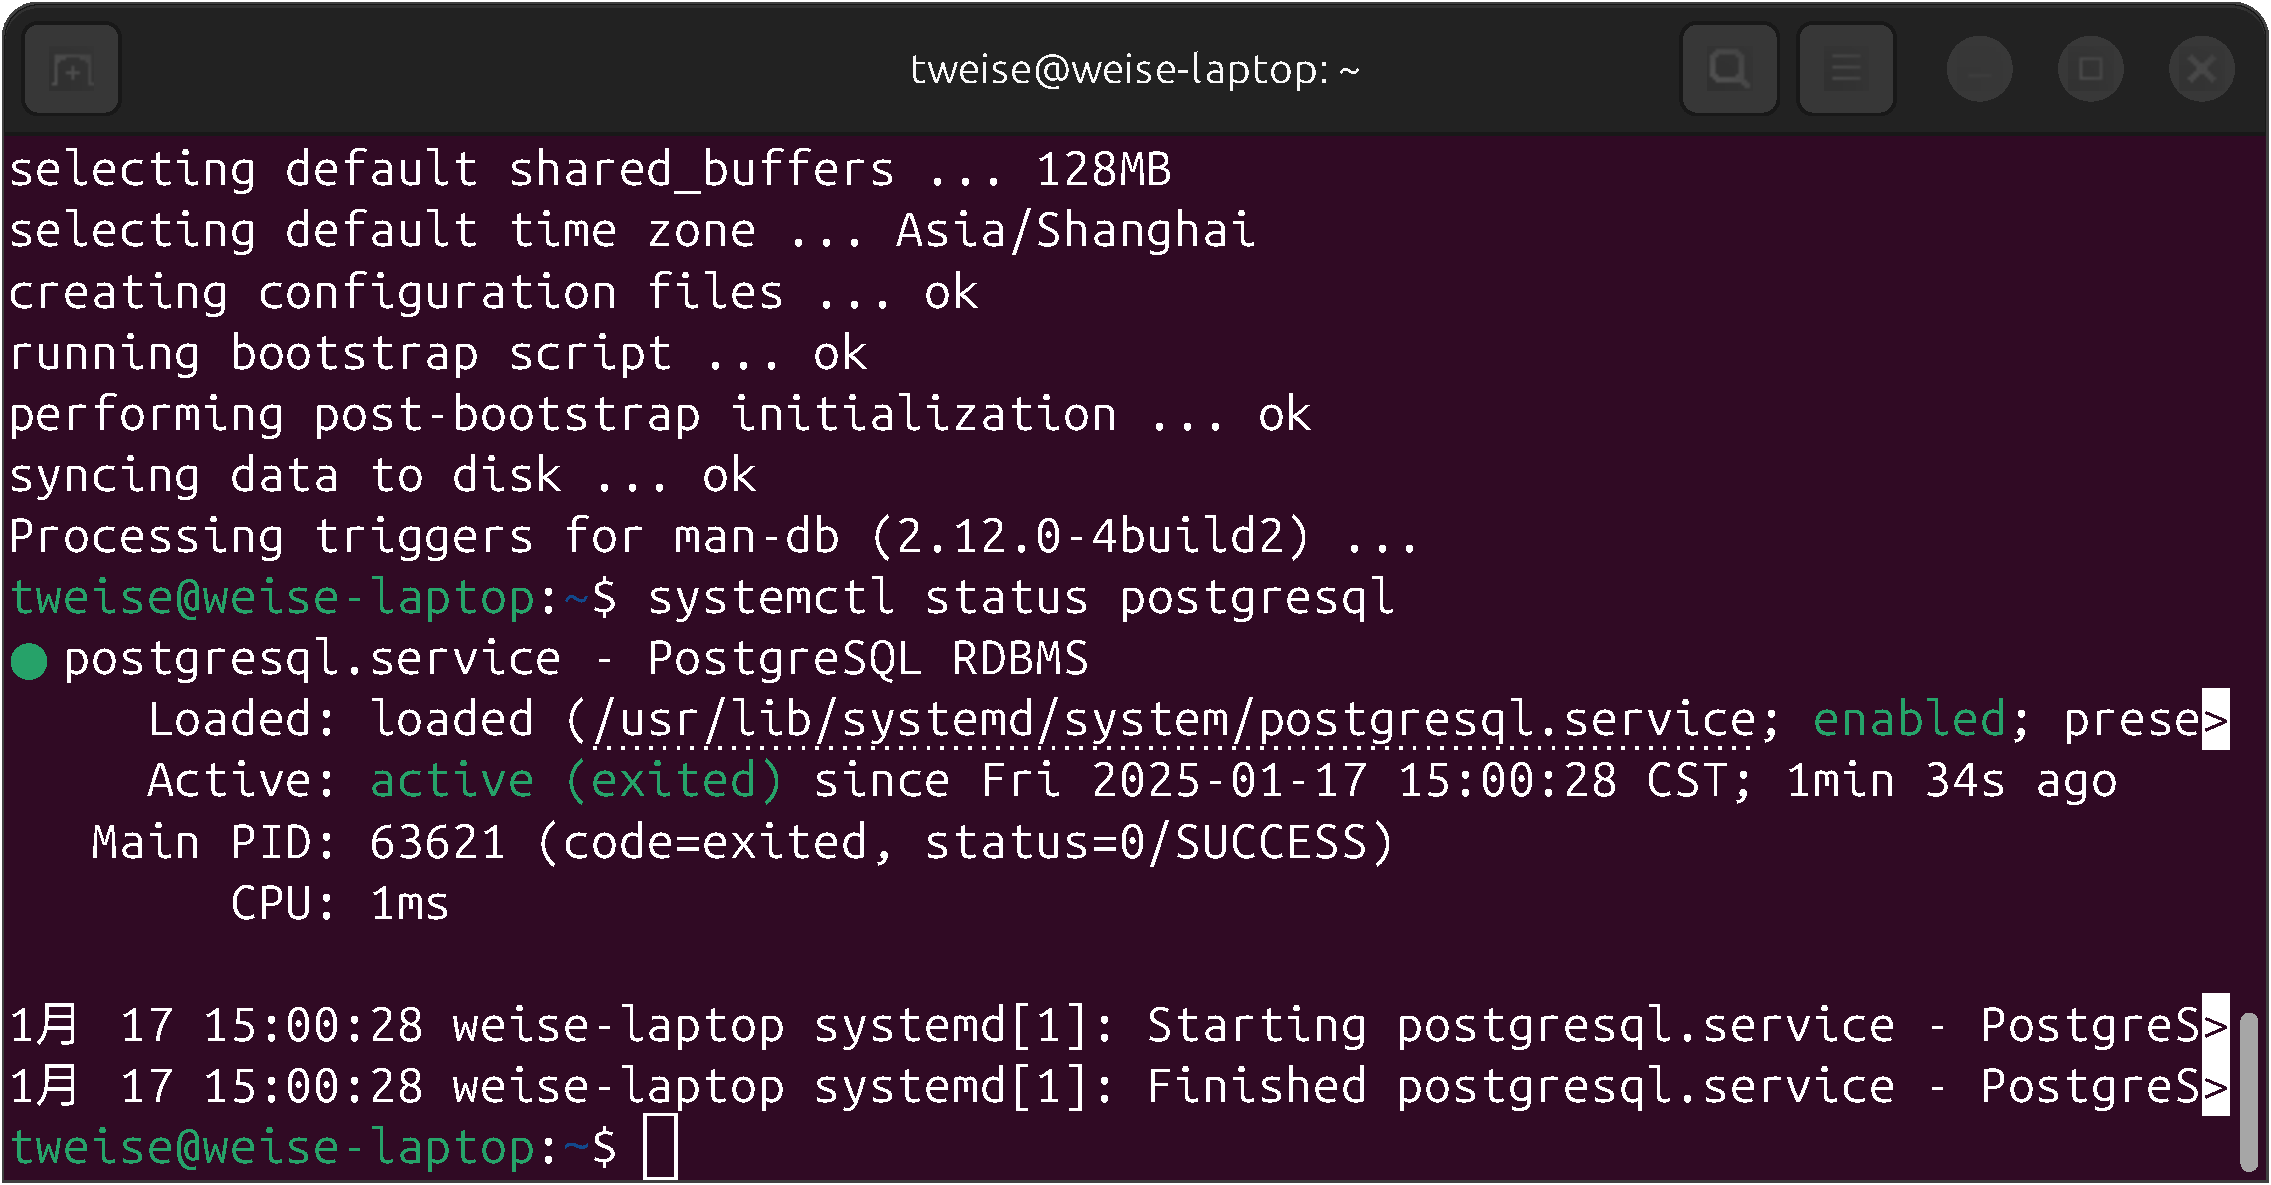
\includegraphics[width=0.7\linewidth]{\currentDir/installingPostgresUbuntu08systemctlCheckStatusQ}}%
%
\floatRowSep
%
\subfloat[][%
\psql\ is the \pgls{client} program that can connect to the \postgresql\ \pgls{server} and that gets installed as well. %
We can check its version by typing \bashil{psql --version} and hitting~\keys{\enter}.%
\label{fig:installingPostgresUbuntu09psqlVersionA}%
]{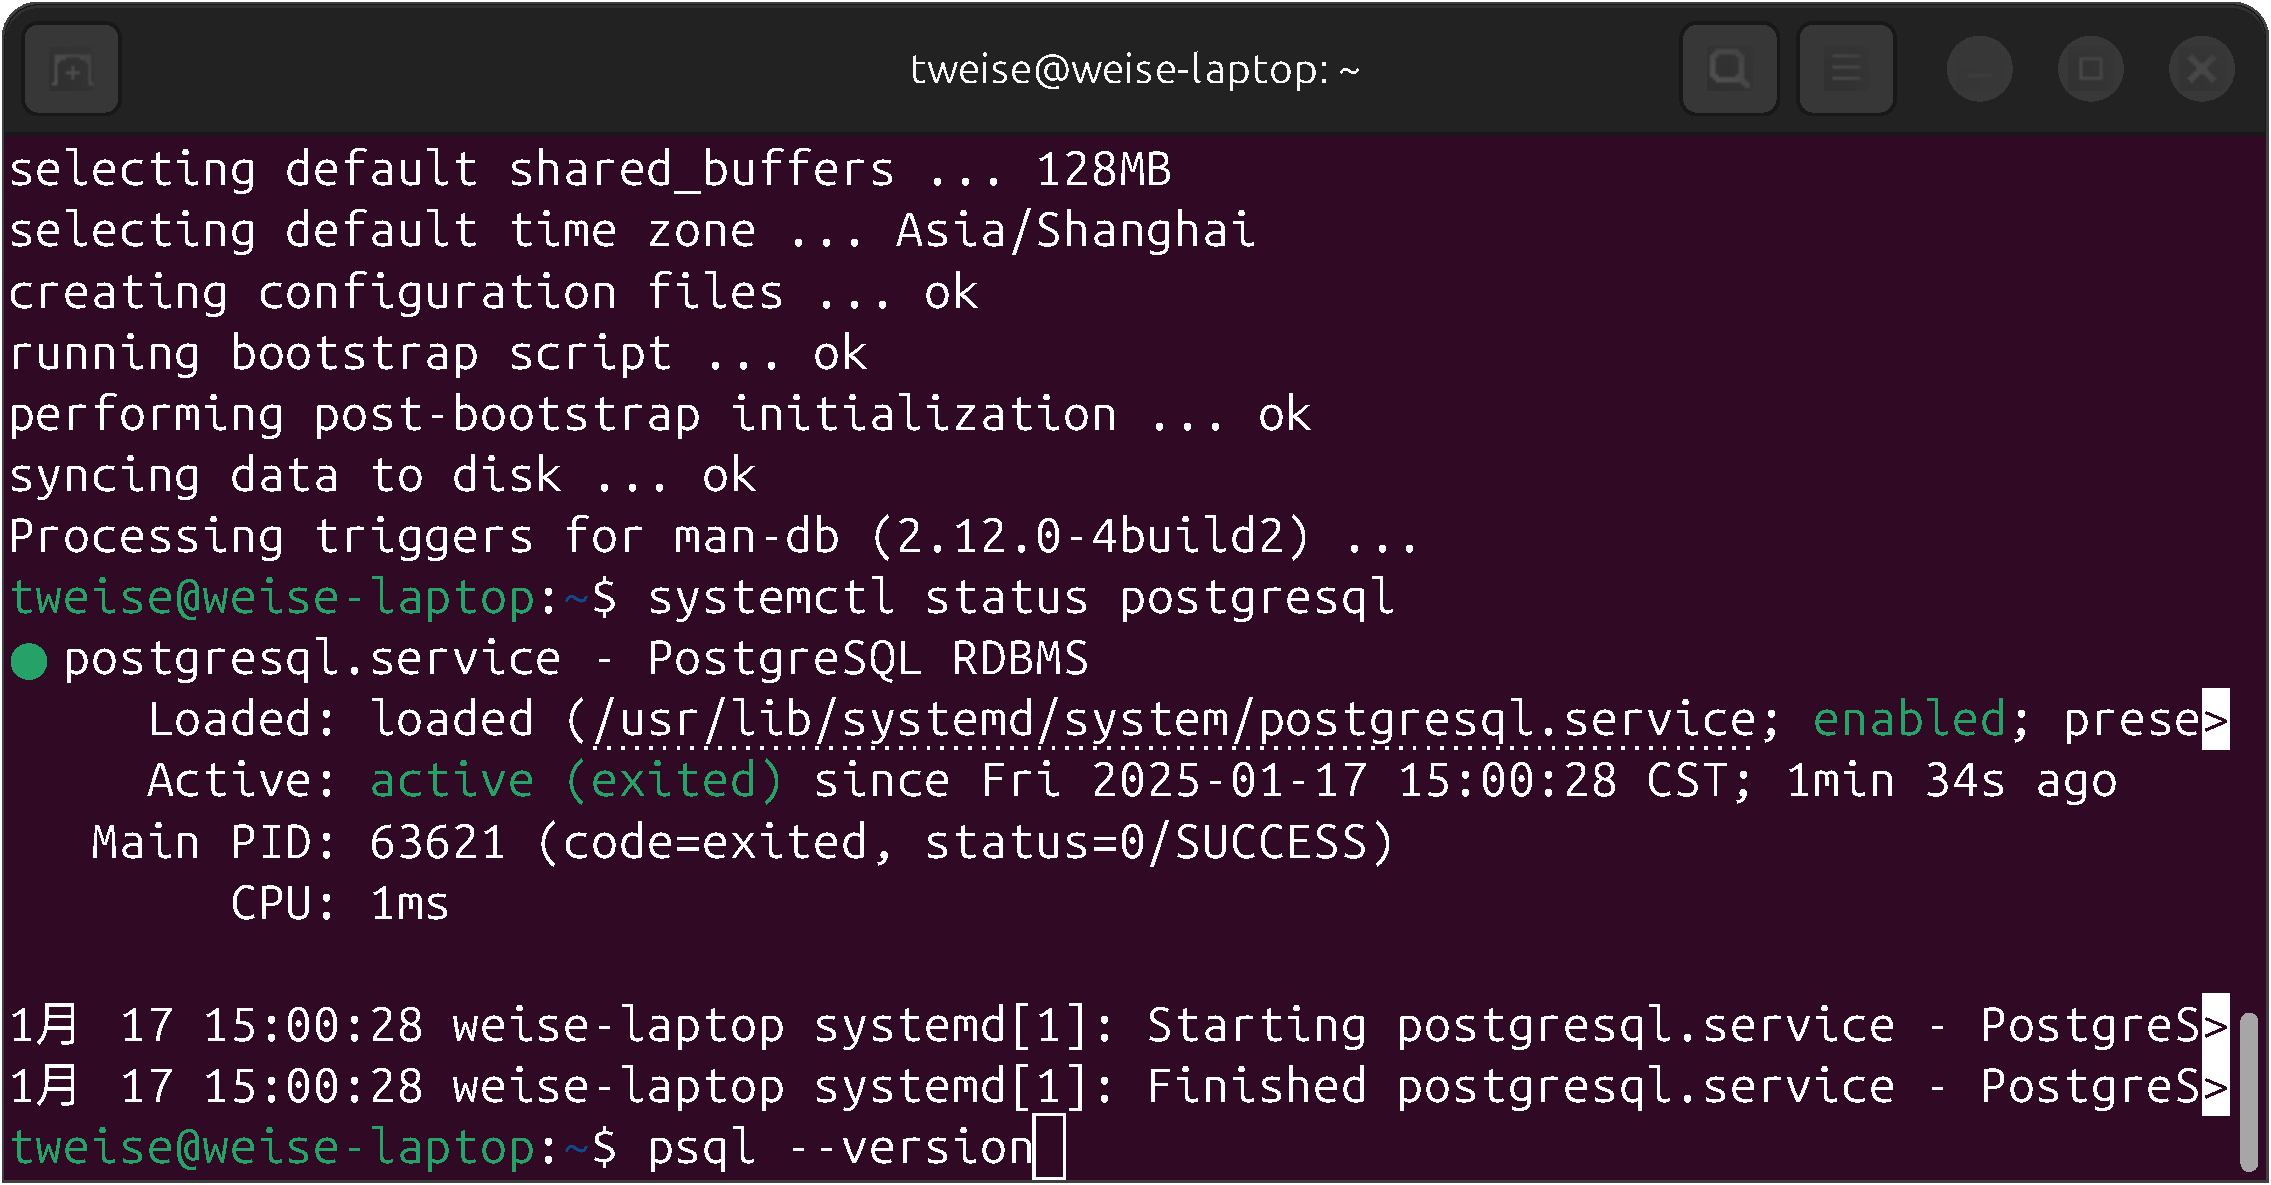
\includegraphics[width=0.7\linewidth]{\currentDir/installingPostgresUbuntu09psqlVersionA}}%
%
\floatRowSep
%
\subfloat[][%
At the time of this writing, I got version~16.6.%
\label{fig:installingPostgresUbuntu10psqlVersionB}%
]{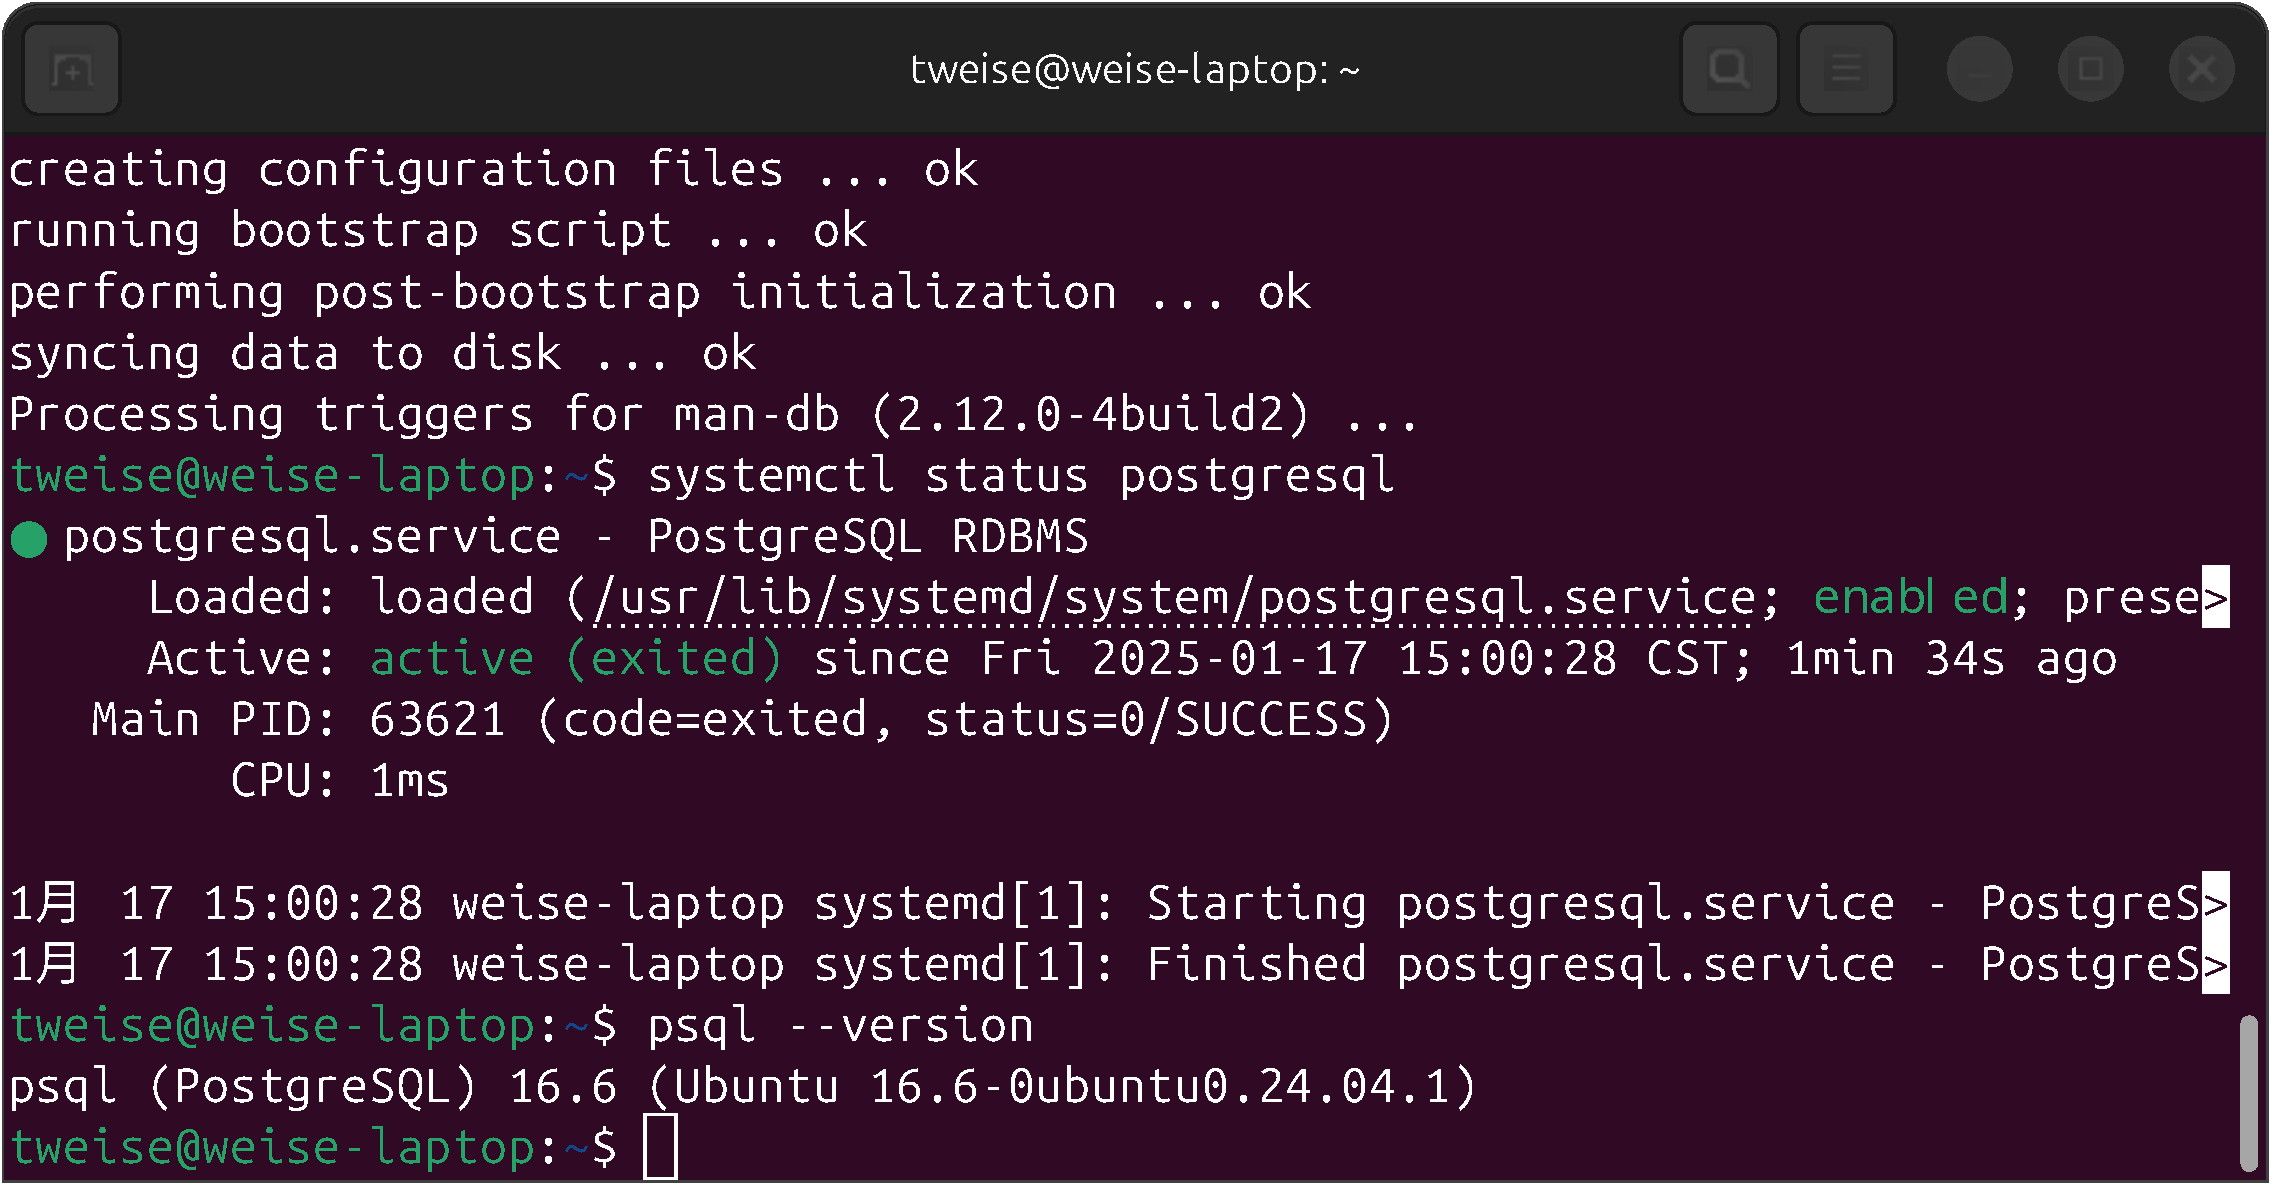
\includegraphics[width=0.7\linewidth]{\currentDir/installingPostgresUbuntu10psqlVersionB}}%
%
%
\caption{Installing \postgresql\ under \ubuntu\ \linux, checking its status, and setting a secure password.}%
\label{fig:installingPostgresUbuntuC}%
\end{figure}%
%
%
\begin{figure}%
\ContinuedFloat
\centering%
%
\subfloat[][%
In order to set a proper password for the \postgresql\ main user \textil{postgresql}, we need to log into \psql\ using \pgls{sudo} privileges, but under the newly created system user \textil{postgres}. %
We do this by writing \bashil{sudo -u postgresql psql} and hit~\keys{\enter}.%
\label{fig:installingPostgresUbuntu11sudoPsql}%
]{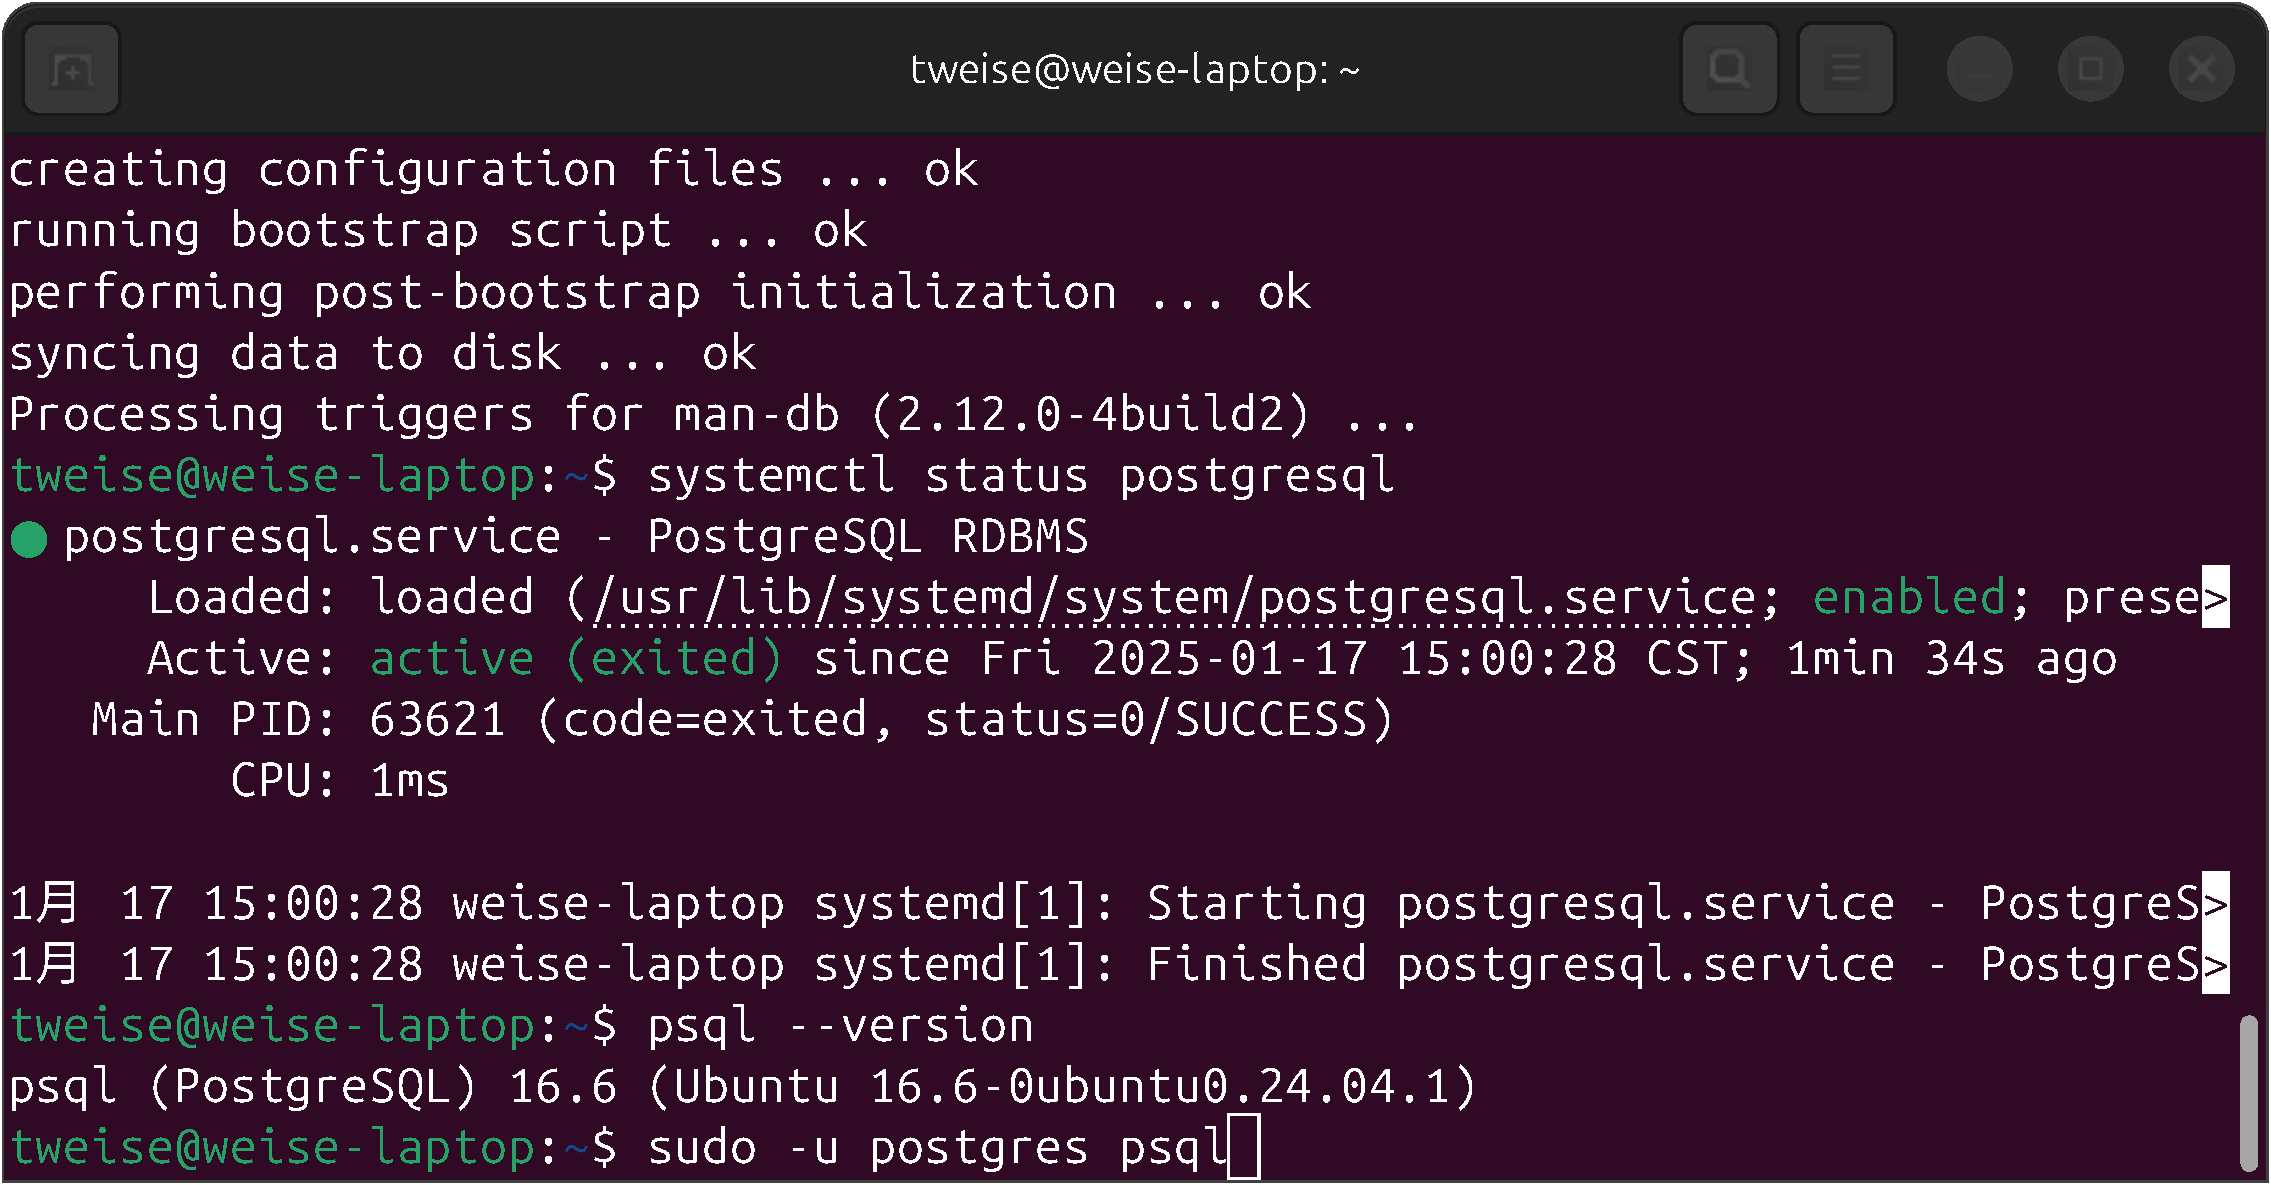
\includegraphics[width=0.7\linewidth]{\currentDir/installingPostgresUbuntu11sudoPsql}}%
%
\floatRowSep%
%
\subfloat[][%
We may or may not need to enter our super user password again\dots%
\label{fig:installingPostgresUbuntu12sudoPsqlPw}%
]{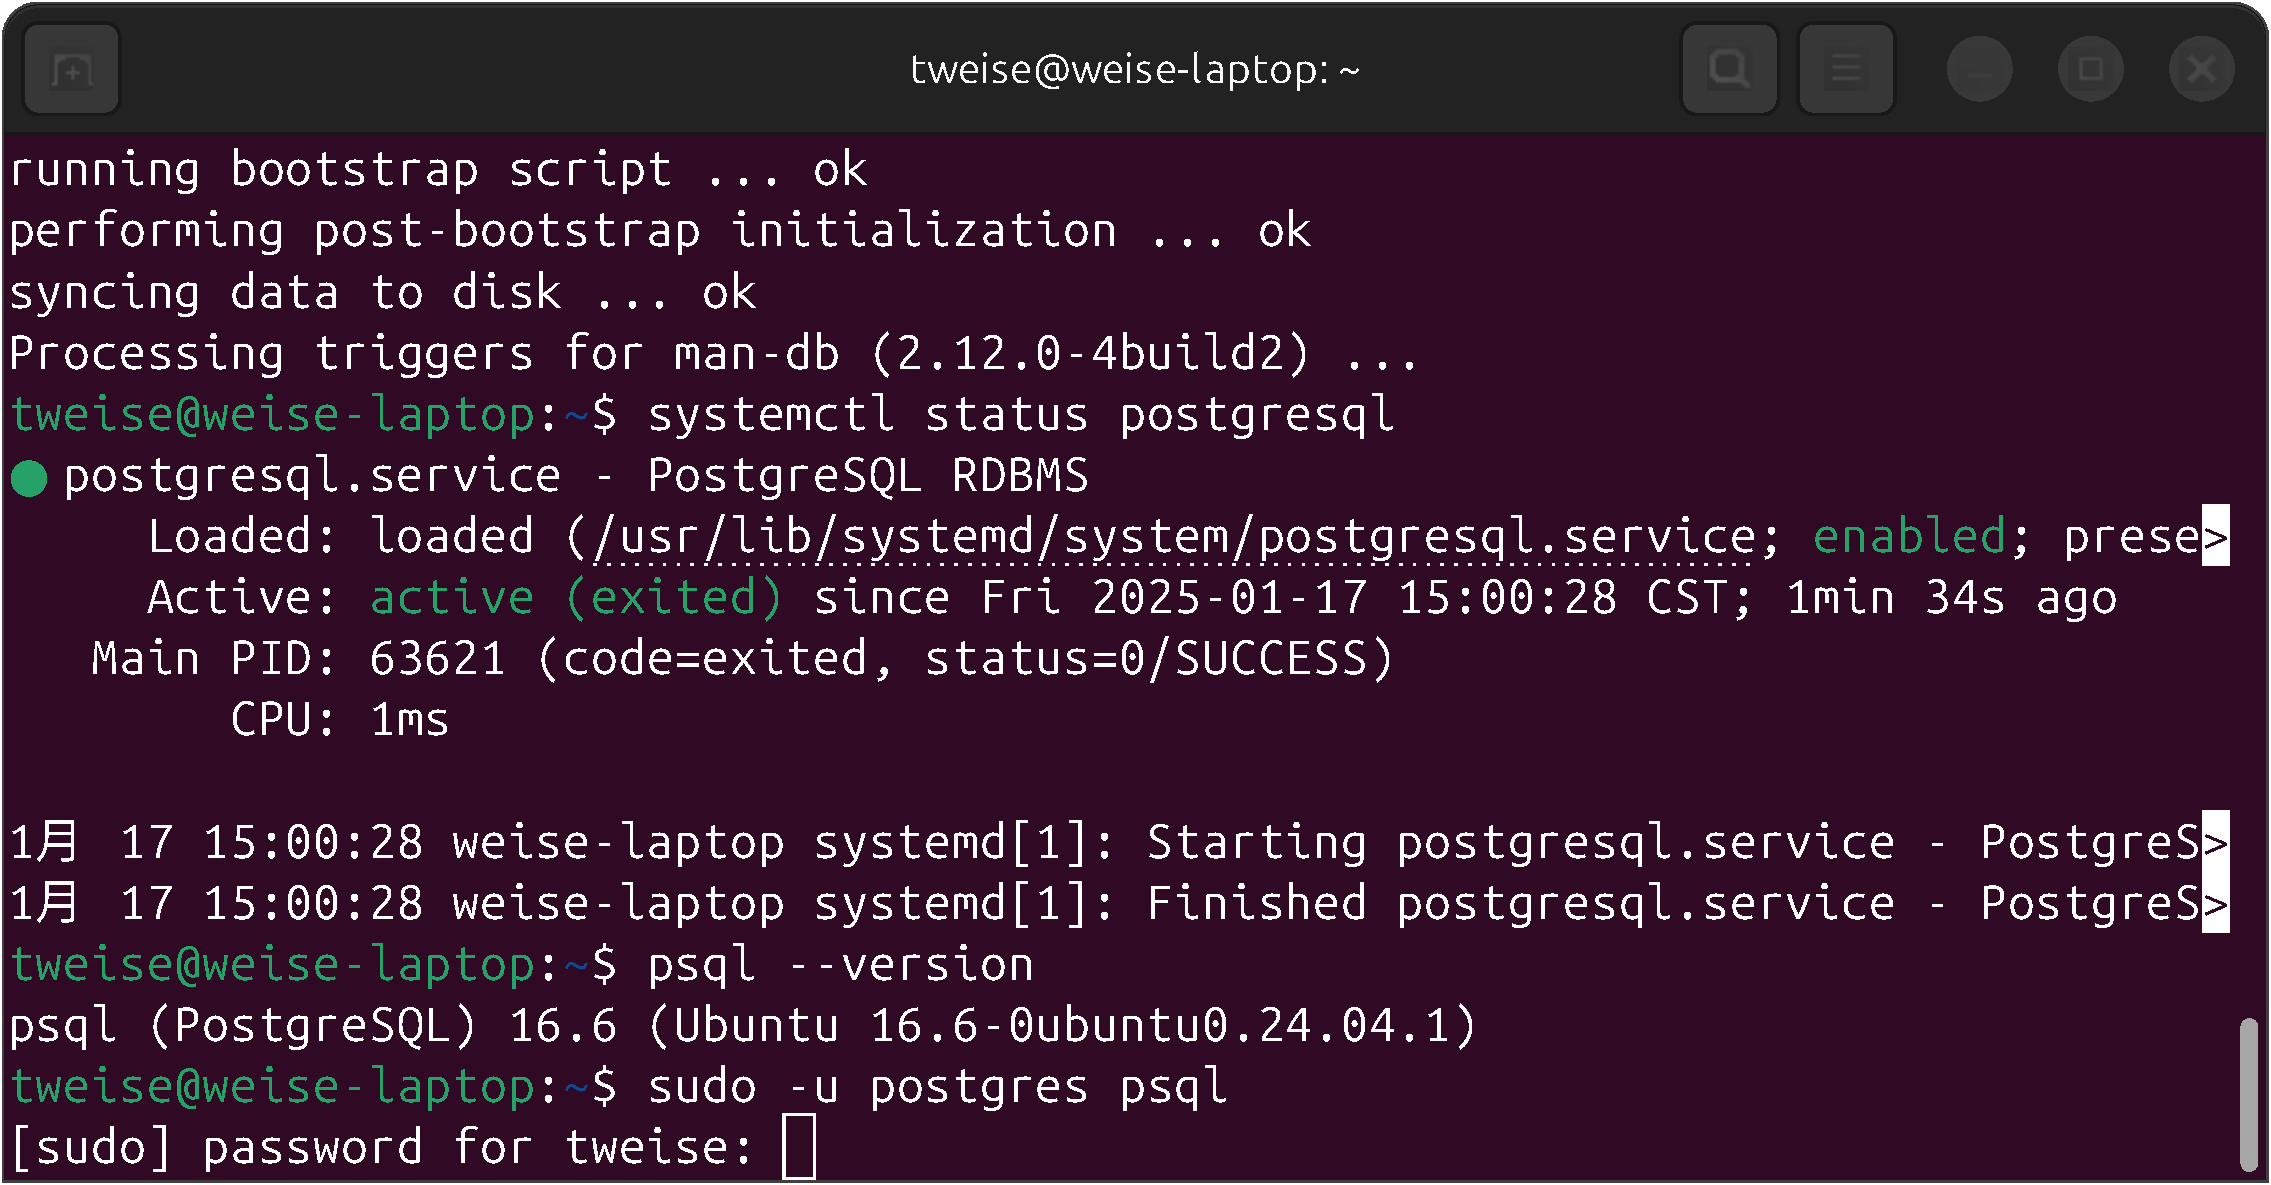
\includegraphics[width=0.7\linewidth]{\currentDir/installingPostgresUbuntu12sudoPsqlPw}}%
%
\floatRowSep%
%
\subfloat[][%
Starting \psql\ like this connects us to the local \postgresql\ \pgls{server}%
\label{fig:installingPostgresUbuntu13PsqlPrompt}%
]{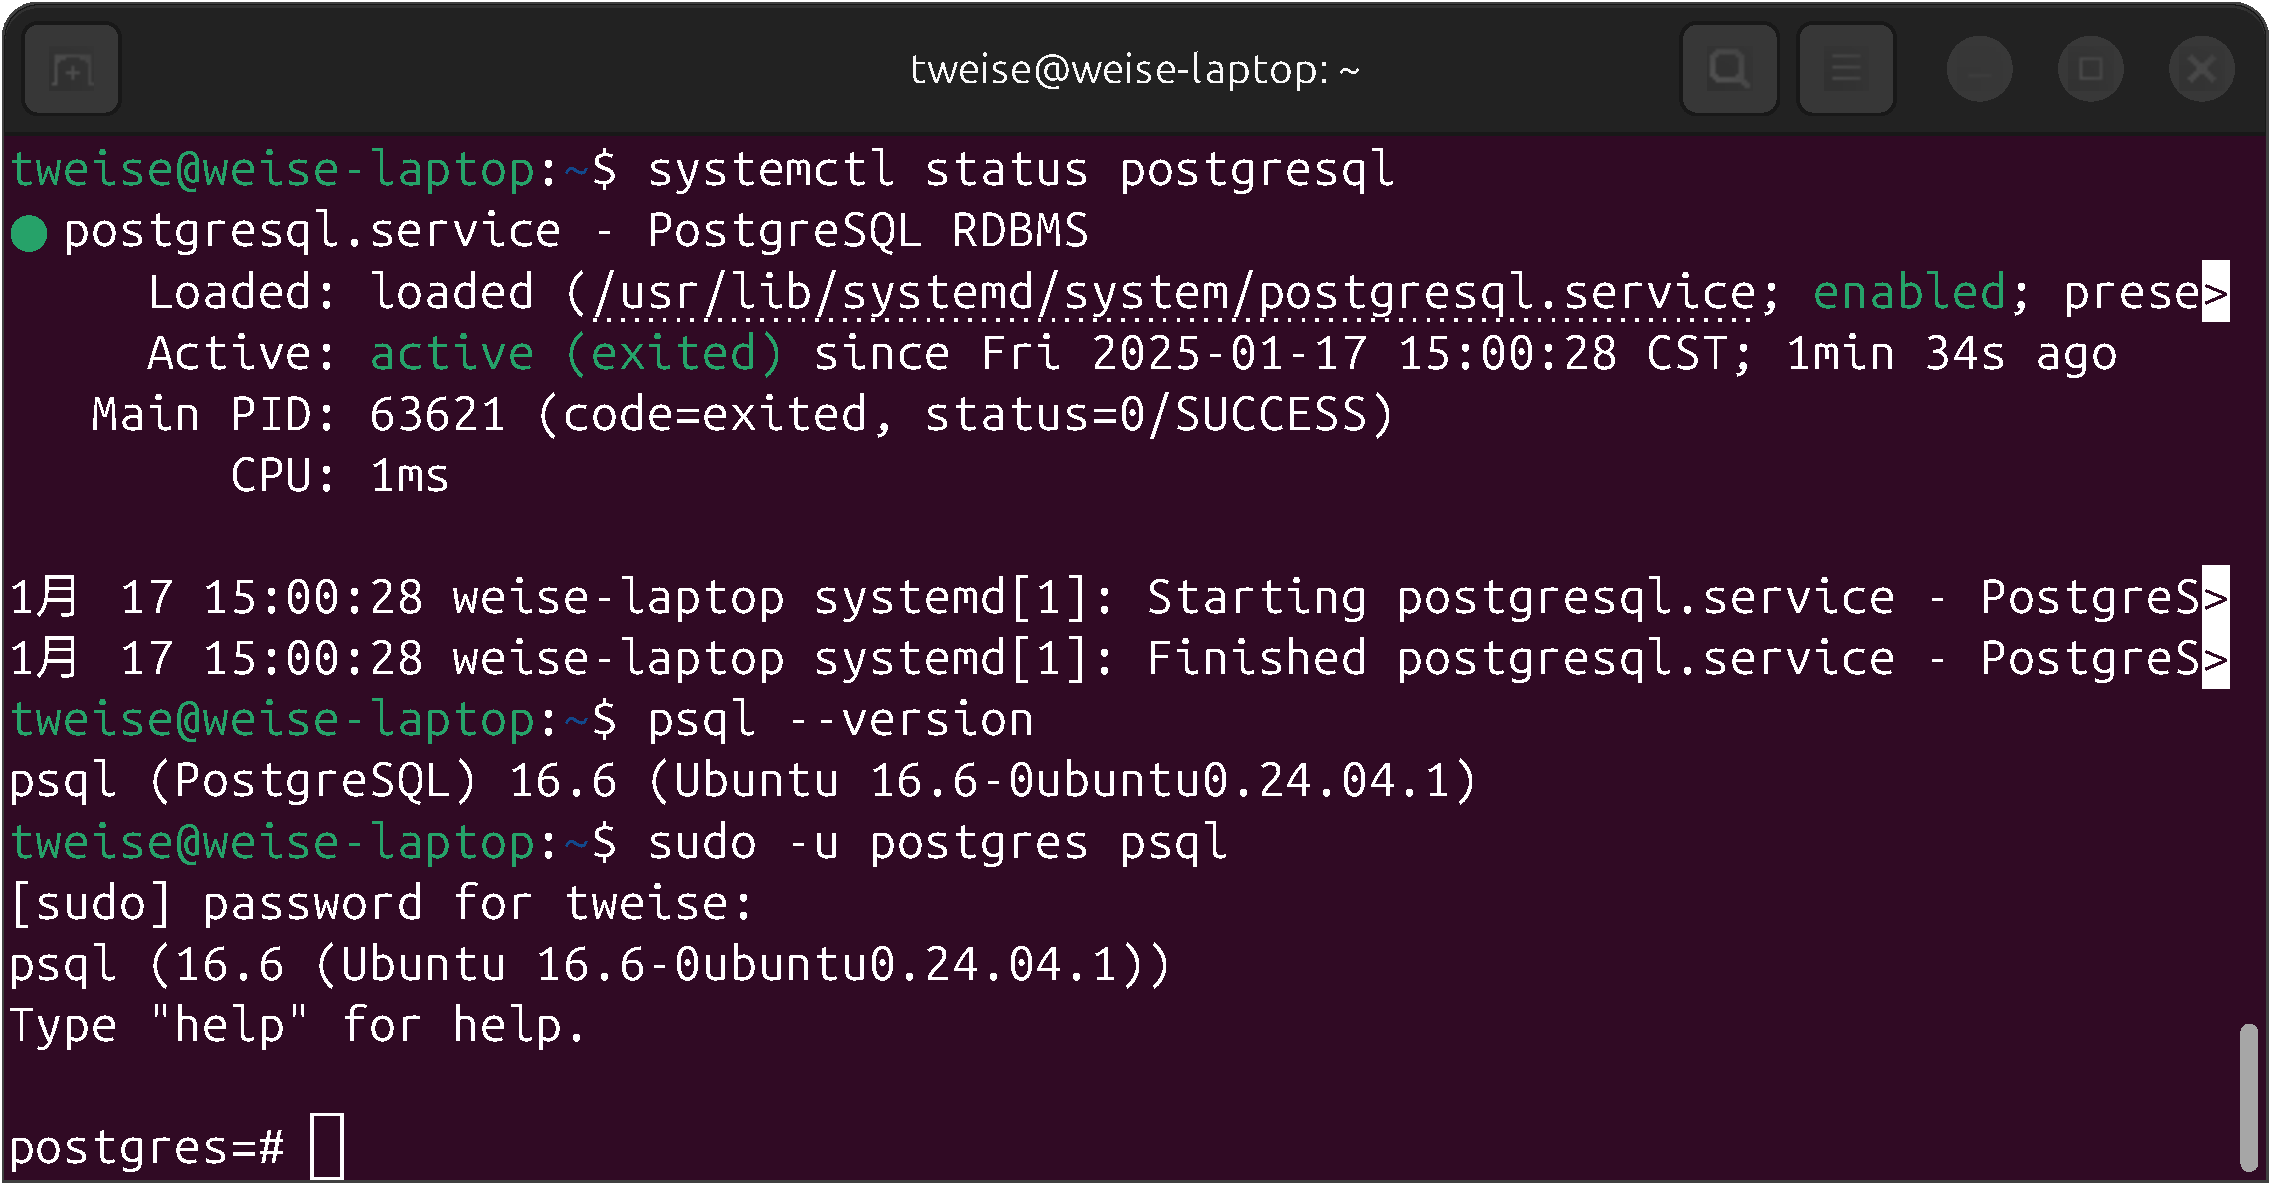
\includegraphics[width=0.7\linewidth]{\currentDir/installingPostgresUbuntu13PsqlPrompt}}%
%
%
\caption{Installing \postgresql\ under \ubuntu\ \linux, checking its status, and setting a secure password.}%
\label{fig:installingPostgresUbuntuD}%
%
\end{figure}%
%
%
\begin{figure}%
\ContinuedFloat
\centering%
%
\subfloat[][%
We can now communicate with the \pgls{dbms} using \sql. %
We use the \sqlIdx{ALTER!USER}\sqlIdx{ALTER!ROLE}\sqlIdx{PASSWORD}\sqlil{ALTER USER postgres PASSWORD 'XXX';} command, where \textil{XXX} is replaced with a secure password. %
In the screenshot, the password is covered by a red rectangle after I replaced it with many~Xs.%
\label{fig:installingPostgresUbuntu14PsqlAlterUserPassword}%
]{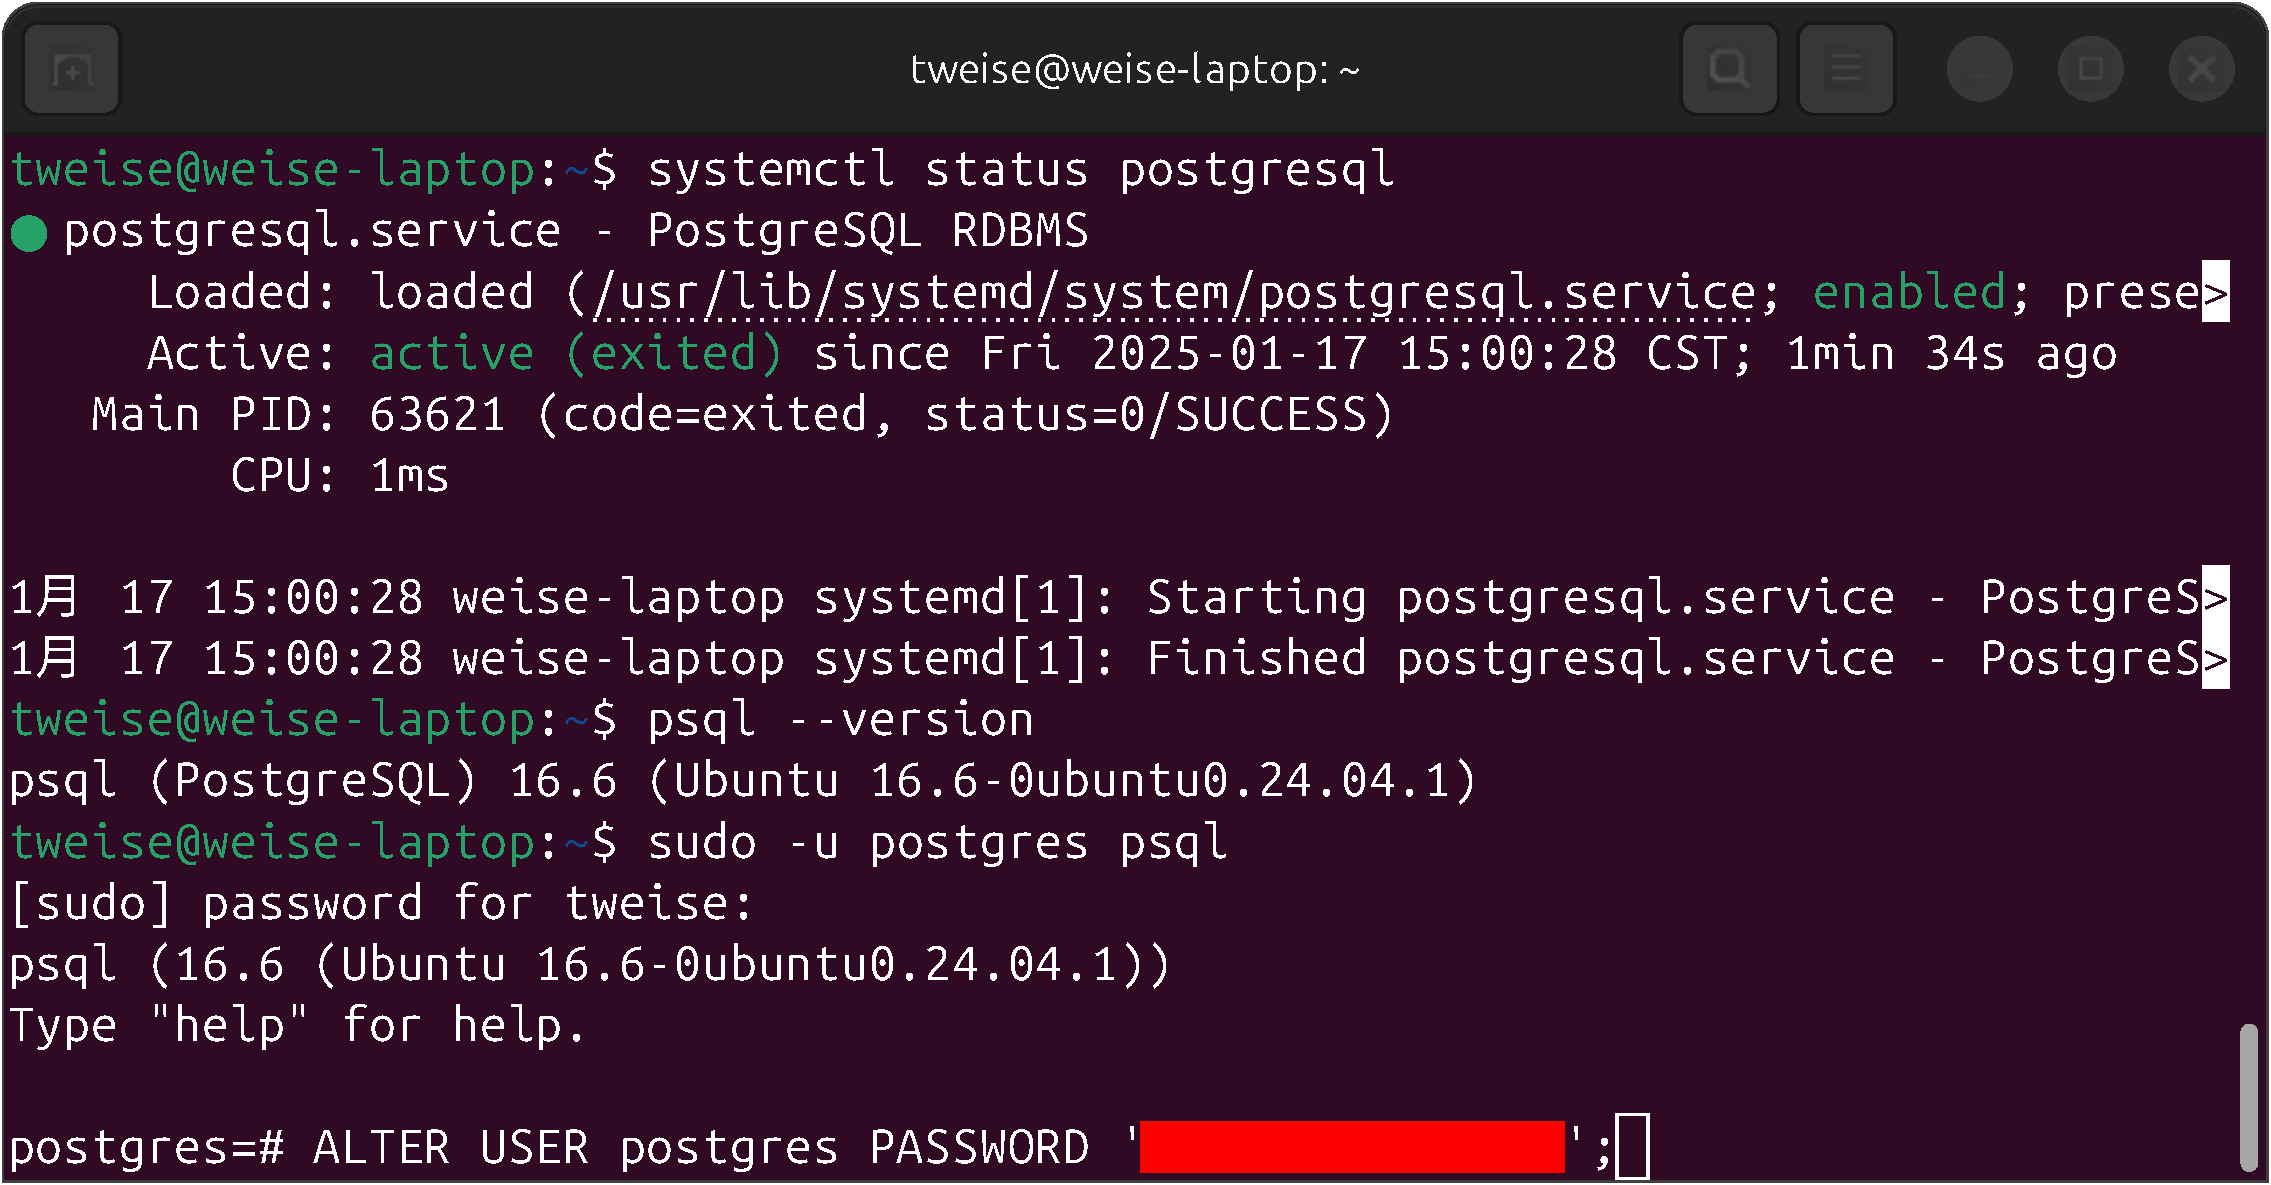
\includegraphics[width=0.7\linewidth]{\currentDir/installingPostgresUbuntu14PsqlAlterUserPassword}}%
%
\floatRowSep
%
\subfloat[][%
After we hit~\keys{\enter}, the system confirms the change by showing the command \sqlil{ALTER ROLE}\sqlIdx{ALTER!USER}\sqlIdx{ALTER!ROLE} back to us. %
From now on, the \pgls{server} main user has a secure password.%
\label{fig:installingPostgresUbuntu15PsqlAlterUserPasswordDone}%
]{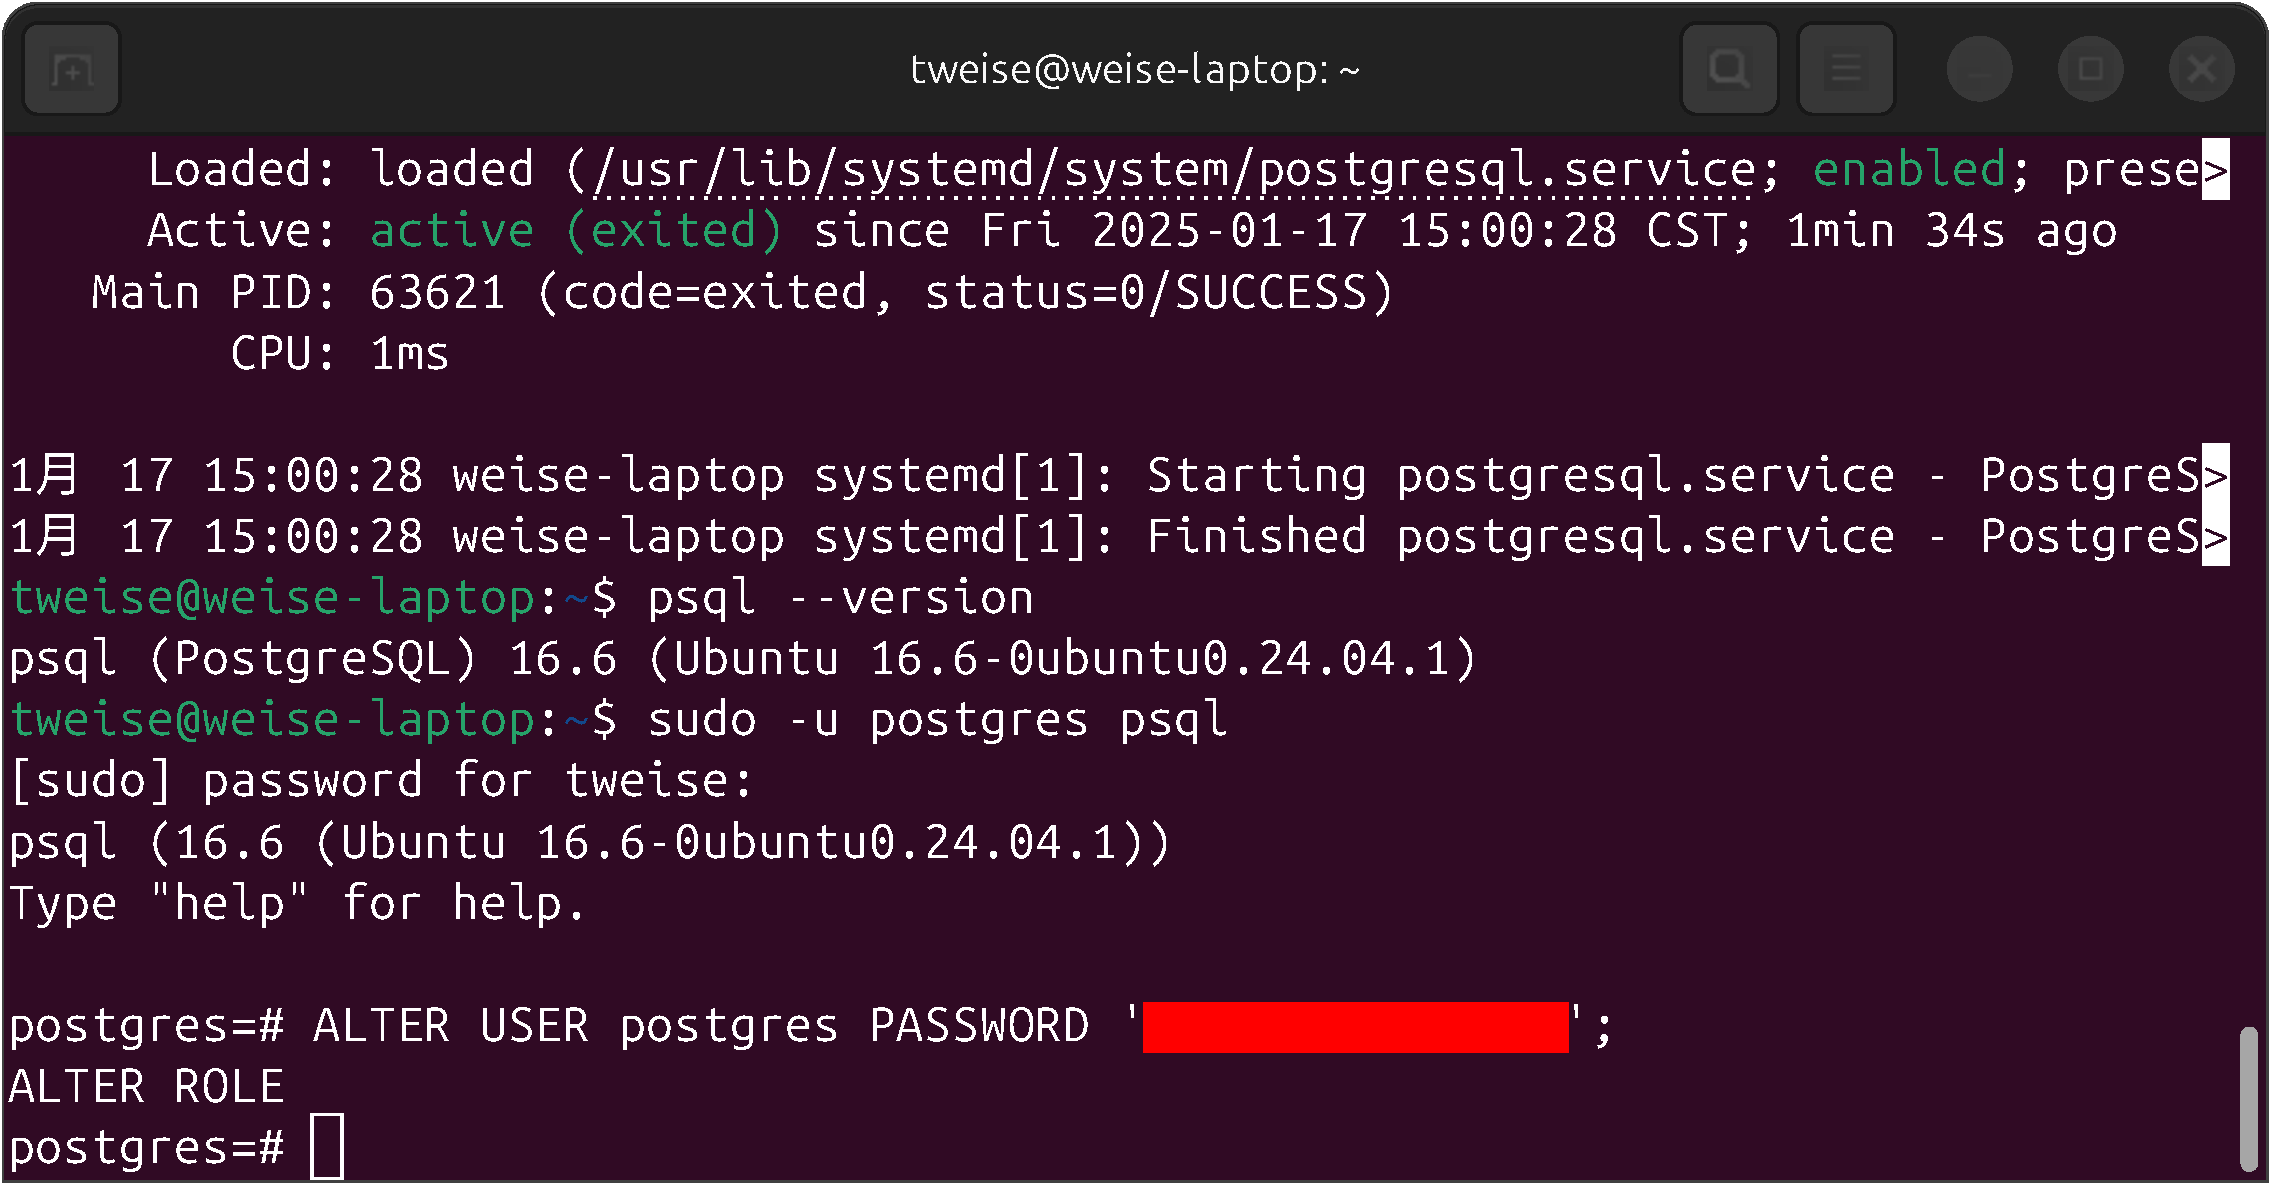
\includegraphics[width=0.7\linewidth]{\currentDir/installingPostgresUbuntu15PsqlAlterUserPasswordDone}}%
%
\floatRowSep
%
\subfloat[][%
We quit \psql\ by typing~\keys{\textbackslash+q+\enter}.%
\label{fig:installingPostgresUbuntu16PsqlQuit}%
]{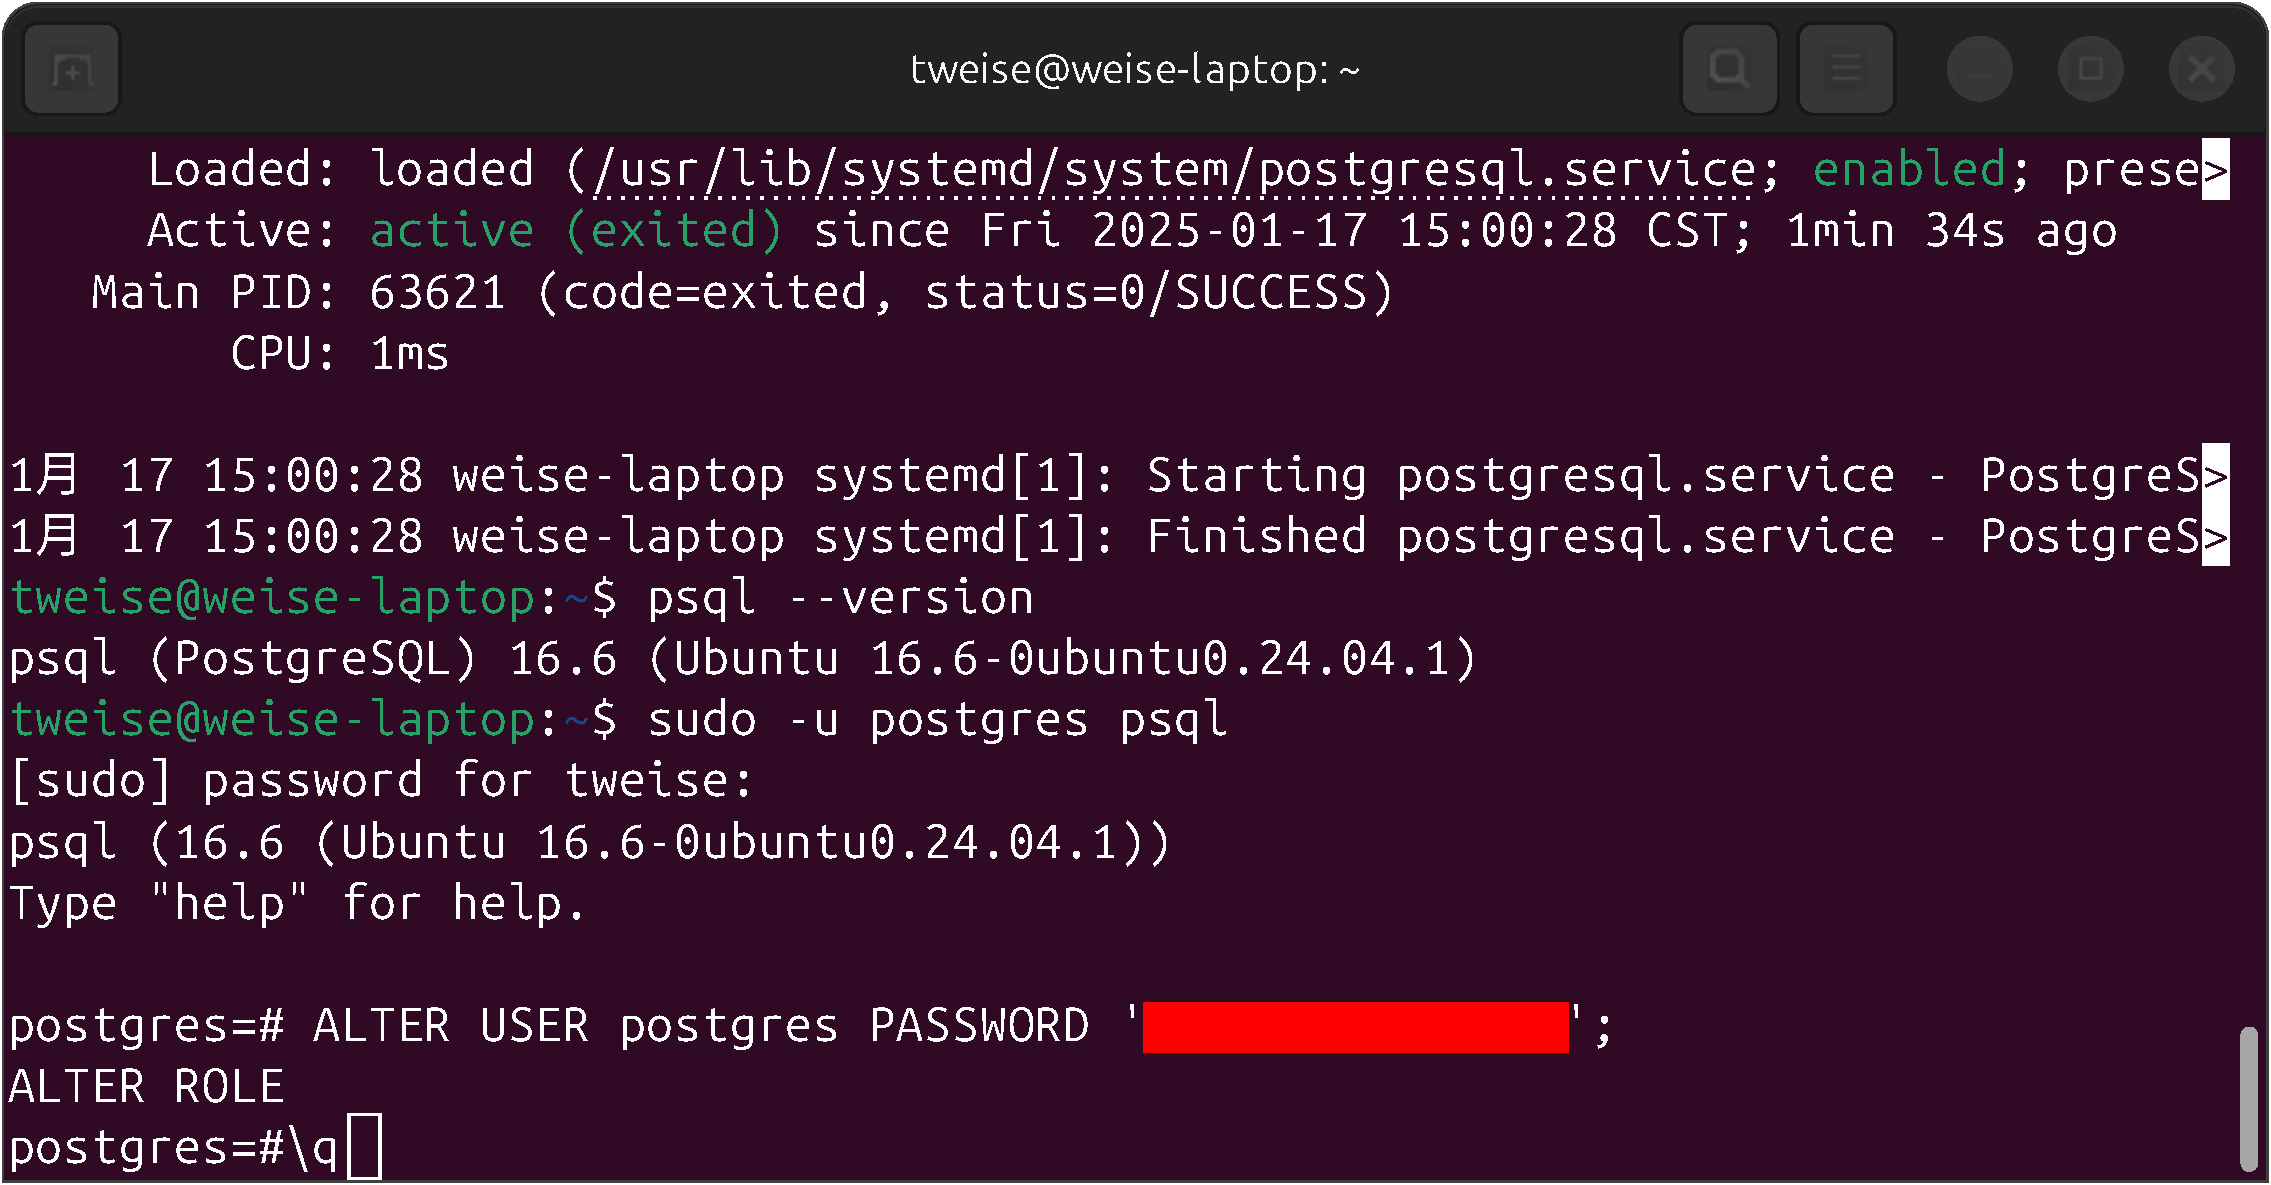
\includegraphics[width=0.7\linewidth]{\currentDir/installingPostgresUbuntu16PsqlQuit}}%
%
%
\caption{Installing \postgresql\ under \ubuntu\ \linux, checking its status, and setting a secure password.}%
\label{fig:installingPostgresUbuntuE}%
%
\end{figure}%
%
%
\begin{figure}%
\ContinuedFloat
\centering%
%
\subfloat[][%
We are finished.%
\label{fig:installingPostgresUbuntu17Done}%
]{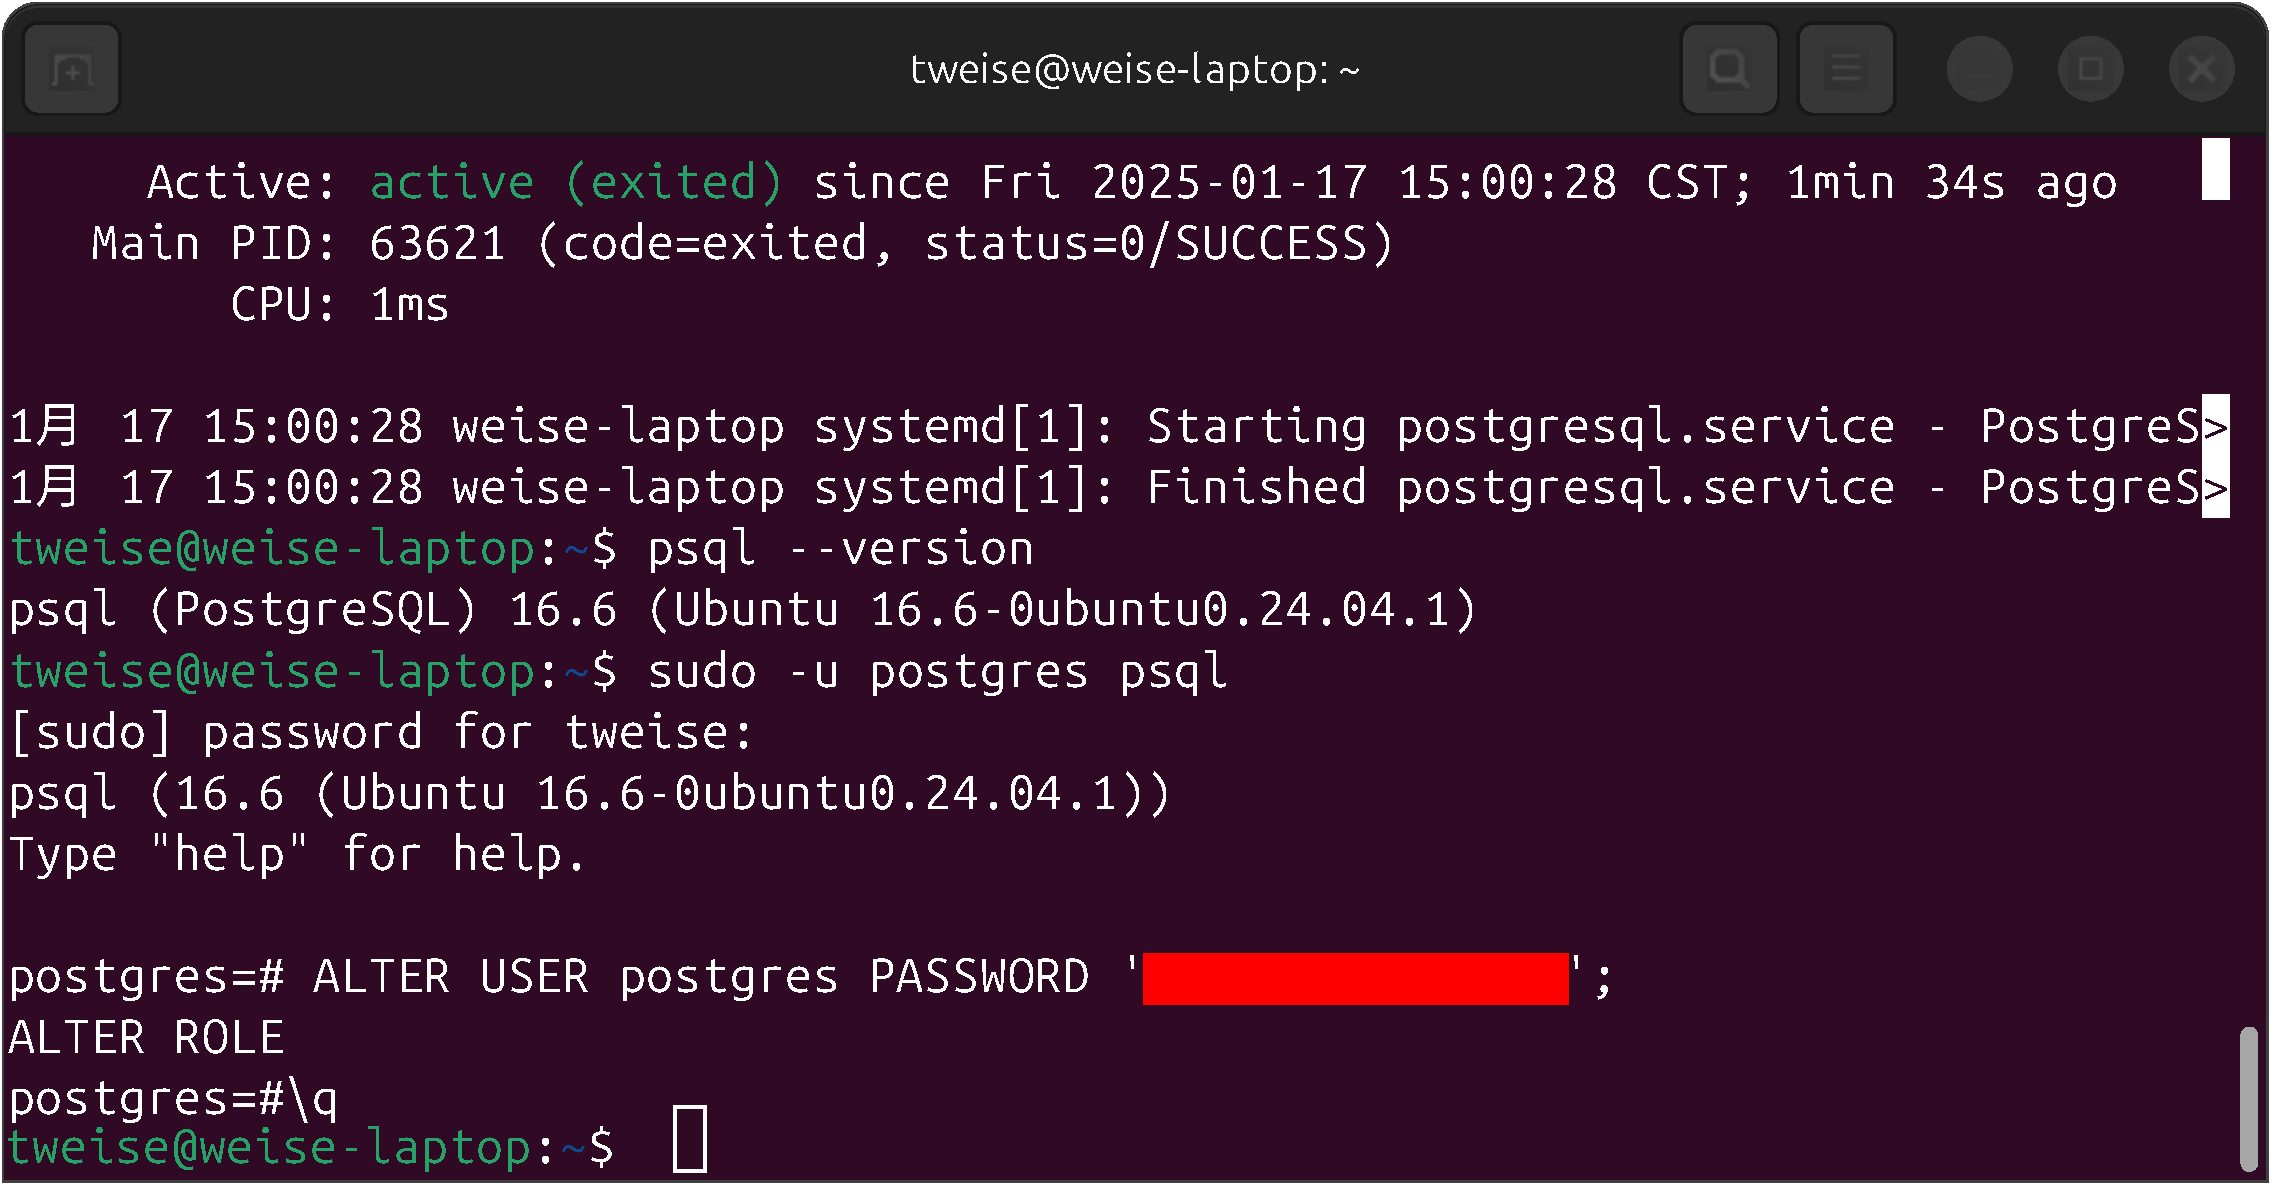
\includegraphics[width=0.7\linewidth]{\currentDir/installingPostgresUbuntu17Done}}%
%
%
\caption{Installing \postgresql\ under \ubuntu\ \linux, checking its status, and setting a secure password.}%
\label{fig:installingPostgresUbuntuF}%
%
\end{figure}%
%
The installation \postgresql\ on \ubuntu\ \linux\ is rather simple.
First, we open a \pgls{bash} \pgls{terminal}, i.e., a window into which we can directly type commands, with \ubuntuTerminal.
Both the \pgls{client} and \pgls{server} program are installed via \bashil{sudo apt-get install postgresql-16}, as shown in \cref{fig:installingPostgresUbuntu01aptGet}.
Notice that we chose to install \postgresql\ version~16, denoted by the \textil{-16}~suffix, but you could probably also pick other versions or just install \textil{postgresql} without version specification.
Either way, this installation method requires super user privileges, which is why we have to start the command with~\pgls{sudo}.
In \cref{fig:installingPostgresUbuntu02pass}, we therefore need to provide our superuser password.

When this is entered and confirmed with~\keys{\enter}, the package manager checks what needs to be installed.
In \cref{fig:installingPostgresUbuntu03yn} it informs us about the package itself and the dependencies that are needed, as well as how much download and space that requires.
It asks us whether we are OK with that, which we confirm by typing~\keys{y+\enter} in \cref{fig:installingPostgresUbuntu04yny}.
Then, the download of the required packages starts.
Once the download completes, the packages are installed.
After this completes in \cref{fig:installingPostgresUbuntu05install}, \postgresql\ is installed and running.

We now want to double-check whether everything went well.
First, we need to investigate whether the \postgresql\ \pgls{DBMS} \pgls{server} is indeed installed and running properly.
We can do this by invoking \bashil{systemctl status postgresql} in \cref{fig:installingPostgresUbuntu06systemctlCheckStatus}.
The output on my laptop computer, given in \cref{fig:installingPostgresUbuntu07systemctlCheckStatusRes}, indicates that the service is up and running.
Notice \textil{active} means that the \pgls{DBMS} is started everytime your computer boots and runs all the time (until you shutdown your computer, that is).
Running this program opens some sort of paginated mode, which we can leave by hitting~\keys{q+\enter} in \cref{fig:installingPostgresUbuntu08systemctlCheckStatusQ}.%
%
\begin{sloppypar}%
If you do not want that, then you disable the service by the command \bashil{sudo systemctl disable postgresql} in the \pgls{terminal}, which again requires \pgls{sudo} privileges.
The \postgresql\ \pgls{server} will then no longer start automatically.
If you want to access it, you then would start it manually via \bashil{sudo systemctl start postgresql}.
After you are done with it, you can stop it by typing \bashil{sudo systemctl stop postgresql}.
If you ever want it to start automatically again, this can be achieved by \bashil{sudo systemctl enable postgresql}.%
\end{sloppypar}%
%
Either way, after a successful installation, the \postgresql\ \pgls{server} service is activated and running.
We now also want to check whether the \pgls{client} program \psql\ was installed correctly.
The \pgls{client} can be run in the \pgls{terminal} and allows us to communicate with the \pgls{DBMS} \pgls{server}.
We therefore type \bashil{psql --version} in \cref{fig:installingPostgresUbuntu09psqlVersionA}, which will print the version of this program after we hit~\keys{\enter}.
The result in \cref{fig:installingPostgresUbuntu10psqlVersionB} shows that the \psql\ \pgls{client} version on my system:~16.6.

Let us now connect to the \postgresql\ \pgls{server} via the \pgls{client} for the first time.
The goal of this exercise will be to set a proper password for the administrative user of our instance the \postgresql\ \pgls{DBMS}.
The installation process created both a \linux\ system user named \textit{postgres} as well as a user of the same name in the \pgls{DBMS}.
The \pgls{DBMS} needs to have its own user and rights management implemented, because we need to be able to grant different programs and users different read and write privileges for a \pgls{db}~(remember \cref{sec:featuresDataPrivacyAndSecurity}).
Thus, we would like the administrative account \textil{postgres} of the \pgls{DBMS} to have some secure password.

We therefore connect the \psql\ \pgls{client} to the \postgresql\ \pgls{server} as superuser impersonating the \bashil{postgres} system user.
This sounds very strange.
I am not even sure whether I explained it correctly.
Either way, we type \bashil{sudo -u postgres psql} into the \pgls{terminal} and hit~\keys{\enter} in \cref{fig:installingPostgresUbuntu11sudoPsql}.
We may get asked to provide the superuser password for our computer again in \cref{fig:installingPostgresUbuntu12sudoPsqlPw}, in which case we simply provide it and hit~\keys{\enter}.

For the first time, we are now in the \psql\ \pgls{client} and are connected to the \postgresql\ \pgls{server}.
We see the prompt \expandafter\textil{postgres=\#} in \cref{fig:installingPostgresUbuntu13PsqlPrompt}.%
%
\begin{sloppypar}%
To set the password for the user (or role) \sqlil{postgres}, we type in \sqlil{ALTER USER postgres PASSWORD 'XXX';}\sqlIdx{ALTER!USER} in \cref{fig:installingPostgresUbuntu14PsqlAlterUserPassword}.
(This is equivalent to \sqlIdx{ALTER!ROLE}\sqlil{ALTER ROLE postgres PASSWORD 'XXX';} in \postgresql.)
This is actually an \sql\ command and we may (or may not) learn later what this exactly means (once and if I get to write such a chapter).
This would set the password to \textil{XXX}.
Obviously, this is not the secure password that we are going to use.
Instead, you will not type \textil{XXX} but a secure password of your choosing.
A password that you shall remember well.
We hit~\keys{\enter}.%
\end{sloppypar}%
%
In \cref{fig:installingPostgresUbuntu15PsqlAlterUserPasswordDone}, we see that this prints \sqlil{ALTER ROLE}\sqlIdx{ALTER!USER}\sqlIdx{ALTER!ROLE} back to us.
It shows us the command that was performed.
We did alter the role (or user) \textil{postgres}.
The new password is set.
You will learn how to use that another time.

For now, we will happily exit the \psql\ \pgls{client} by typing~\keys{\textbackslash + q + \enter}.
In \cref{fig:installingPostgresUbuntu16PsqlQuit}, we quit the \pgls{client} this way.
In \cref{fig:installingPostgresUbuntu17Done}, we then are back in our normal \bash\ \pgls{terminal}.
We have finished and validated the \postgresql\ installation.
And we have set a proper password for the administrator account~\textil{postgres}.%
%
\FloatBarrier%
\endhsection%
%
